\documentclass[12pt]{article}
\usepackage{fontspec}

\usepackage{afterpage} % For deferring content to a specific later page
\usepackage{xcolor}
\usepackage{mathrsfs}

\usepackage{tocloft}  % Include this package to customize the ToC
\usepackage[titletoc]{appendix} % Helps manage appendices

\setmainfont{Times New Roman} % Times New Roman, Arial, Calibri

\usepackage{setspace}
\setstretch{1.15}

% Set paragraph indentation to zero
\setlength{\parindent}{0pt}

% Add some space between paragraphs
\setlength{\parskip}{0.5em} % Adjust the amount of space to your liking

\usepackage{pdflscape}

\usepackage{longtable}
\usepackage{enumitem}
\usepackage{graphicx}
\usepackage{caption}

% Define a command to set the font size and make it bold
\newcommand{\captionfonts}{\fontsize{10pt}{12pt}\selectfont\bfseries}

\DeclareCaptionLabelSeparator{dash}{ - }

% Apply the custom font command to the captions
\captionsetup[figure]{
    font=small,
    format=plain,
    labelfont=bf,
    textfont=bf,
    labelsep=dash,
    justification=centering
}

\captionsetup[table]{
    font=small,
    format=plain,
    labelfont=bf,
    textfont=bf,
    labelsep=dash,
    justification=centering
}

\DeclareCaptionFont{bf}{\captionfonts}
\captionsetup[figure]{font=bf}
\usepackage{float}
\usepackage{placeins}
\usepackage[backend=biber, style=numeric, sorting=none]{biblatex}
\addbibresource{references.bib}

\usepackage{geometry}
\geometry{top=2.5cm, bottom=2.5cm, left=2.6cm, right=2.6cm}

\usepackage{pdfpages}

\usepackage{listings}
\usepackage{xcolor}
% Define colors
\definecolor{codegreen}{rgb}{0,0.6,0}
\definecolor{codegray}{rgb}{0.5,0.5,0.5}
\definecolor{codepurple}{rgb}{0.58,0,0.82}
\definecolor{backcolour}{rgb}{0.95,0.95,0.92}

% Setup the listings package
\lstdefinestyle{mystyle}{
    backgroundcolor=\color{backcolour},
    commentstyle=\color{codegreen},
    keywordstyle=\color{magenta},
    numberstyle=\tiny\color{codegray},
    stringstyle=\color{codepurple},
    basicstyle=\ttfamily\footnotesize,
    breakatwhitespace=false,
    breaklines=true,
    captionpos=b,
    keepspaces=true,
    numbers=left,
    numbersep=5pt,
    showspaces=false,
    showstringspaces=false,
    showtabs=false,
    tabsize=2
}

\usepackage{array} % For better column formatting

\lstset{style=mystyle, language=Python}
\captionsetup[lstlisting]{
    labelsep=dash,
    font=bf
}

\usepackage{amsmath} % For mathematical features

% Allow changes to internal LaTeX commands
\makeatletter
% Redefine the tag form to be bold and without parentheses
\renewcommand{\tagform@}[1]{\textbf{#1}}
\makeatother

\renewcommand{\theequation}{\thesection.\arabic{equation}}
\renewcommand{\thefigure}{\thesection.\arabic{figure}}

\usepackage{gensymb}
\usepackage{nomencl}
\usepackage{chngcntr}
\usepackage{amssymb}
\usepackage{hyperref}
\usepackage{hyperref}
\usepackage{hyperref}
\usepackage{hyperref}
\usepackage{hyperref}
\usepackage{hyperref}
\usepackage{hyperref}
\usepackage{hyperref}
\usepackage{hyperref}
\counterwithin{figure}{section}
\counterwithin{equation}{section}
\counterwithin{table}{section}

\title{Identifying Dynamic Systems with Probabilistic Numerics}
\author{Harvey Walton}
\date{\today}

%Repeated Text
\newcommand{\ndiFigCaption}[1]{The rectangle method for finding the #1 bound of the integral of the standard Gaussian (normal) distribution between -2 and 1.}

\hyphenpenalty=700
\exhyphenpenalty=700

\makenomenclature

% Define nomenclature groupings
\renewcommand{\nomgroup}[1]{%
    \ifthenelse{\equal{#1}{G}}{\item[\textbf{Greek Symbols}]}{%
        \ifthenelse{\equal{#1}{L}}{\item[\textbf{Latin Symbols}]}{}}}

\setlength{\nomlabelwidth}{2.5cm}
%\renewcommand{\nomlabel}[1]{\textbf{#1}\hfil} % Bold the symbols and right-align
%\setlength{\nomitemsep}{-\parsep} % Reduce the space between items

\begin{document}
    \pagenumbering{roman}

    \thispagestyle{empty}
    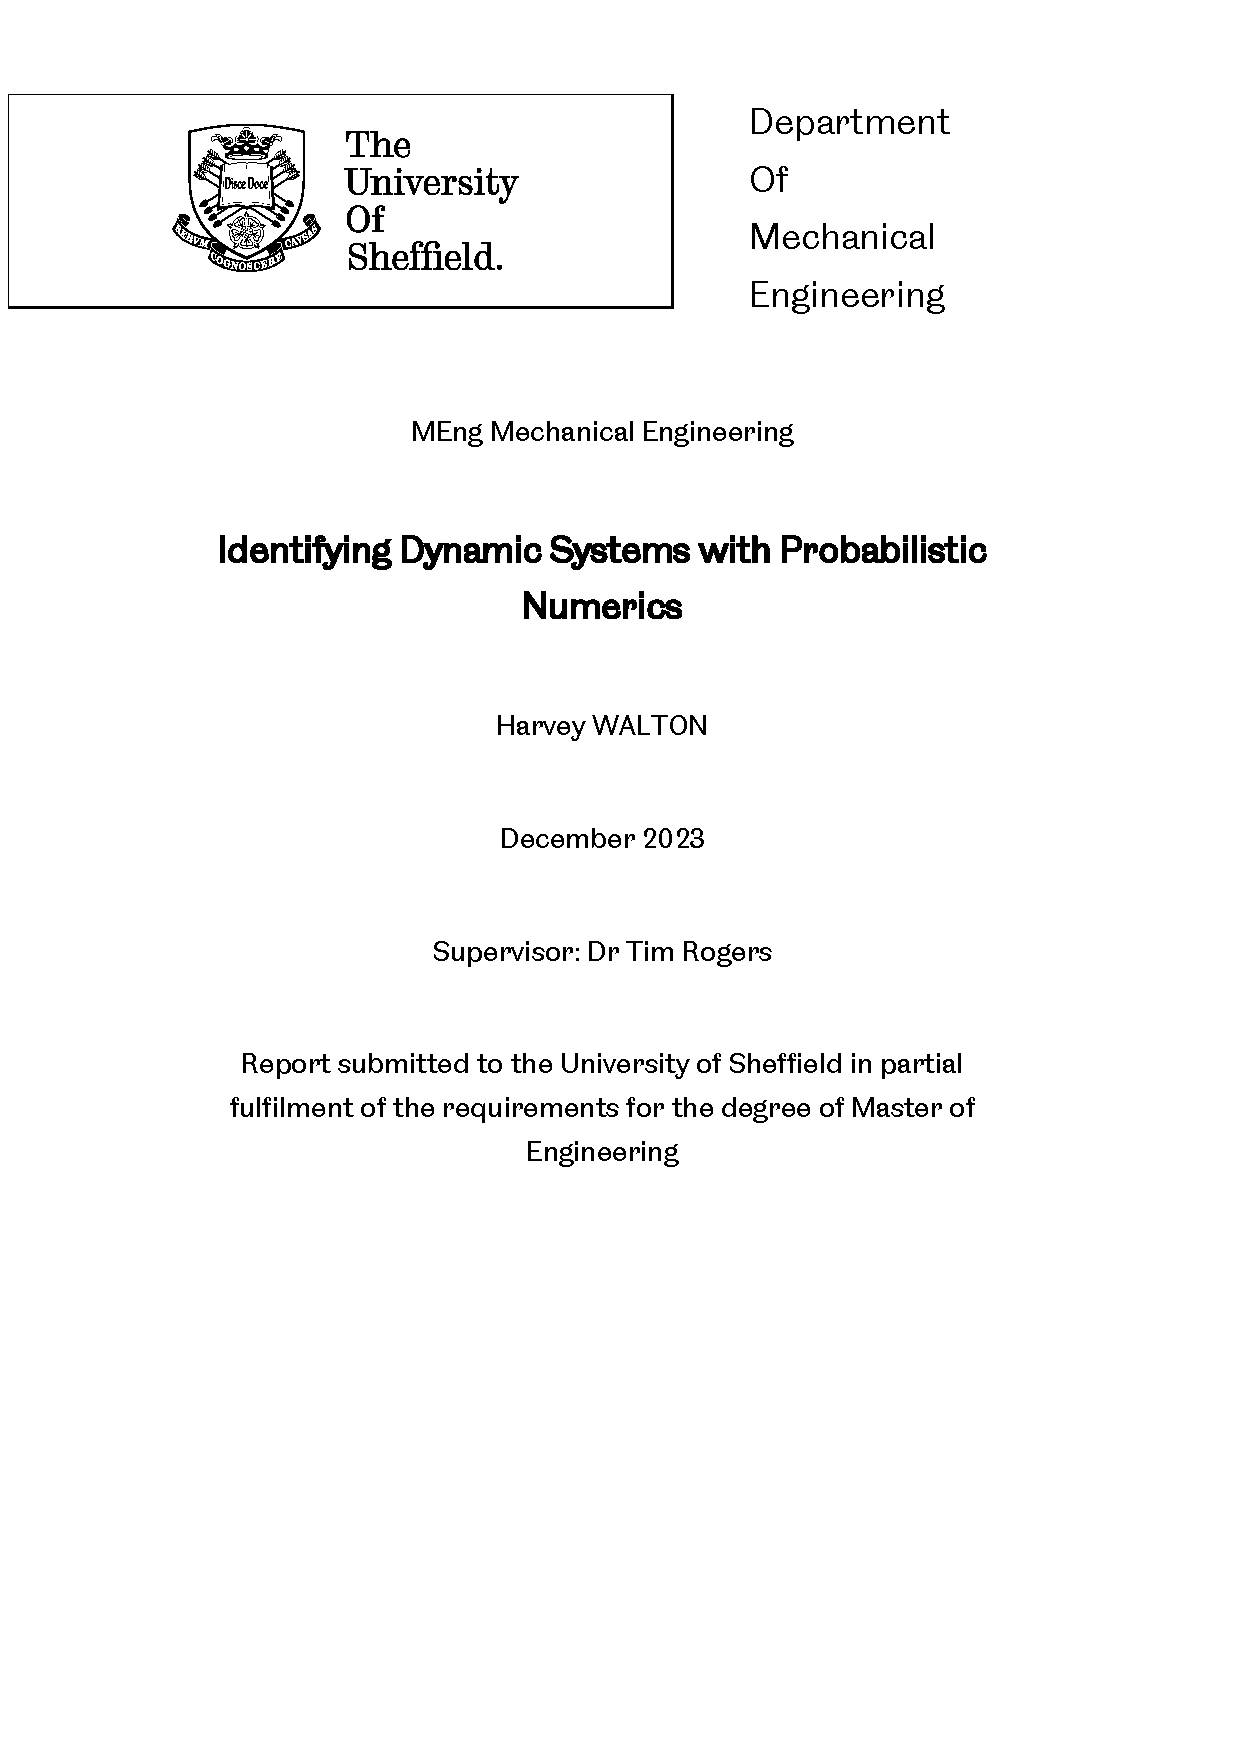
\includepdf[pages=1, frame, scale=1.09, pagecommand={}, offset=0 -35]{figures/titlepage.pdf}

    \section*{Summary}
    In mechanical engineering, the field of dynamics studies how systems, like structures and fluids, respond and evolve over time under varying forces.
    Being able to characterise these systems by identifying their dynamic properties and parameters helps to design structures that last longer before failing from fatigue, and that are less likely to fail structurally from excessive excitation under external forces.
    The identification of dynamic systems often uses the ``Frequency Response Function'', which relies on the ``Fourier transform'' to convert data from a function of time to a function of frequency.
    This paper explores a new paradigm of ``probabilistic numerics'' over traditional numerical methods that allows the Fourier transform to be performed through the use of a Gaussian Process (GP) machine learning model.
    The model showed significantly better robustness to noise compared to the industry standard Fast Fourier Transform (FFT), exhibiting an improved Mean Squared Error in magnitude versus the true analytical Fourier transform by a factor of $9.66$.
    Therefore, it could allow dynamic systems to be identified more accurately in across industry where data is noisy, from aviation to renewable power generation.
    Furthermore, the model had several promising features that made it more versatile in this context.
    Most notably, the fact that the time domain input data need not be evenly spaced enabled it to detect frequencies that would be above the Nyquist limit of what would be detectable by an equivalent FFT of the same number of datapoints sampled evenly across the same time period.
    This makes the model most suitable in industrial contexts where there are constraints to the amount of data that can be collected due to cost, availability, or limited memory.
    However, the computational speed of this GP model is currently orders of magnitude slower than the FFT, so before it can be a viable alternative in practice, it would need development to allow it to scale better to large datasets.

    \printnomenclature

    \newpage
    \tableofcontents
    \newpage

    \pagenumbering{arabic}

    \section{Background and Understanding of the Problem}

    \subsection{Dynamic Systems}
    In mechanical engineering, the field of dynamics studies how systems, like structures and fluids, respond and evolve over time under varying forces.
    These forces can range from aerodynamic pressures to impacts from waves or road irregularities.
    Excessive vibration or oscillation of machinery is known to reduce service life and in extreme cases cause catastrophic failure.
    Therefore, by studying these dynamic systems they could be designed to perform better, be safer and to have lower maintenance costs.
    However, the field of dynamics is far from being mastered since there are many types of problems that cannot yet be solved.

    To begin with, here are some examples of dynamic systems:
    \begin{enumerate}[listparindent=\parindent]
        \item Firstly, a motorcycle suspension system is a combination of springs, dampers and linkages that connect the motorcycle chassis to its wheels.
        Its primary purpose is to keep the tyres in contact with the ground, and without proper suspension, the tyres would lose traction when encountering bumps especially when braking, accelerating or cornering~\cite{UTI2020MotorcycleSuspension}.
        It is designed to allow some relative motion between the chassis and the wheels in order to absorb impacts while at the same time trying to maintain its equilibrium position, and zero velocity (both relative to the chassis).

        The dampers in the suspension produce a force proportional to the velocity that acts to slow the wheel down.
        Viscous dampers do this by pushing a liquid though a small orifice as the wheel moves.
        Damping can be optimised (or made ``critical'') by bringing the system back to equilibrium after a disturbance as fast as possible.
        Too little damping, and the wheel will overshoot and oscillate back and forth before reaching equilibrium.
        Too much damping, and although the wheel will not oscillate, it will reach equilibrium more slowly than optimal.

        Similarly, the springs create stiffness in the system that produces a force with a magnitude proportional to the displacement of wheel which acts to return the wheel to its equilibrium position.
        Too high of a stiffness means that the system will not have enough time to absorb the impact softly, but too low means that the bike's responses to steering inputs are slow and unreactive.

        Studying this dynamic system could allow for the prediction of behaviour based on varying these parameters.
        This would enable optimisation without trial and error, conserving resources during the research and development phase of the product lifecycle.

        \item Secondly, offshore wind turbines are known to experience high cycle fatigue due to a relentless random forcing the waves that repeatedly crash against the base of its tower.
        This is a phenomenon that causes any micro-defects to grow into cracks over time due to cyclic loading below the elastic limit of the material, which reduces the life of the structure due to increased risk of mechanical failure.

        The rate at which this occurs increases with the amplitude of the stresses in the structure, which in turn increase with the amplitude of oscillation in response to this cyclic loading.
        If a periodic force is applied to any system with a specific frequency known as a resonant frequency, the amplitude of the oscillation may become very large even for a small amplitude force, leading to an excessive rate of high cycle fatigue.
        The same can happen in the case of the wind turbine that receives a random force with an \textit{average} frequency similar to this resonant frequency.
        It is even possible for the stresses in a structure to become so large that they exceed the ultimate tensile strength of the material, causing a sudden mechanical failure and the collapse of the turbine.

        Therefore, to make structures safer and reduce maintenance costs, it would be valuable to be able to model their dynamic properties (such as this resonant frequency) from system parameters (such as the stiffness of the tower) so that the frequencies at which they occur can be designed away from the expected frequencies of the periodic forces.

        \item Finally, an aircraft wing bends in response to aerodynamic forces.
        However, the forces themselves change as the wing twists and bends.
        The interdependence of these two effects creates complicated interactions that are difficult to model accurately.
        But it is important to do so because if at high airspeed, energy from the wing forcing is added to the system faster than it can be dissipated, the positive feedback loop can lead to a phenomenon called aerodynamic flutter where the oscillations become larger and larger until they cause catastrophic failure.
    \end{enumerate}

    \subsection{Identifying Dynamic Systems}

    So, dynamic systems have parameters such as mass ($m$), damping coefficient ($c$) and stiffness ($k$) which are fundamental characteristics of the system.
    ``Forwards modelling'' is when the observable behaviour of the system, known as the system properties, are predicted from the system parameters using physical laws.
    These properties include the resonant frequencies which are the forcing frequencies that produce a peak in amplitude of excitation, the mode shapes which are the shapes of oscillations at peaks in systems with multiple degrees of freedom, and the damping ratios which compare the damping coefficient to that of critical damping at each resonant frequency.

    \nomenclature[L22]{$m$}{The mass}
    \nomenclature[L03]{$c$}{The damping coefficient}
    \nomenclature[L181]{$k$}{The stiffness}

    Often a distinction is made between linear and nonlinear systems.
    Only linear systems comply with the principle of superposition, which states that ``when two or more waves simultaneously pass through a point, the disturbance at the point is given by the sum of the disturbances each wave would produce in absence of the other waves''~\cite{StudyComSuperposition}.
    This means that if you double the input force over time, the response over time is exactly double, but otherwise identical.
    This is not the case for nonlinear systems (such as the aircraft wing in the example above) where non-compliance with the principle of superposition causes the system properties to distort as the magnitude of the input force is increased.
    This, in turn, causes the response to become highly complex and chaotic, meaning that it is highly sensitive to initial conditions.
    This is why forward modelling is currently too difficult for systems that are non-linear.

    Unfortunately, everything is non-linear in real life.
    Only in rare cases are systems close enough to being linear that they can be approximated as such.
    What's worse is that even if a model did exist to solve the nonlinear system, it would be of no use because typically not even the system parameters are known to be able to input them into the model.
    This is why the field of dynamics has not been mastered, and all that can currently be done for medium to highly non-linear systems - \textit{which is almost all systems} - is to take real life data measurements from an existing system and identify the system properties and parameters that best fit the observed data through what is known as ``inverse modelling''.
    However, even this process is fraught with issues and uncertainty.

    \subsection{Classically Quantifying Uncertainty with Error Bounds}
    Identifying system properties and parameters using this inverse modelling approach results in values that are not exact, but have an uncertainty associated with them that comes from multiple sources.
    The first source of uncertainty is noise that is always present to some degree in sampled input data due to the measuring devices - typically accelerometers - that are used to capture the force input and corresponding response from the system.
    Furthermore, even if the true input and response could be sampled exactly, the non-identifiability problem states that since there are multiple sets of system parameters that could give the same set of observed outputs, it's impossible to uniquely determine them~\cite{Grabowski2023}.
    Similarly, many algorithms make use of mathematical objects (such as matrix pseudoinverses) which have multiple alternatives - any of which could be used - where the correct choice is subjective.
    This noise and lack of uniqueness is reflected in the outputted system properties and parameters as uncertainty.

    Time passes continuously forever, and the governing equations of dynamic systems are defined mathematically in the continuous domain.
    In theory, these could be solved ``analytically'' to give an exact mathematical solution in the continuous domain, but in practice, data sampled from the real world is usually discrete, meaning that it is defined by a finite set of points separated by finite time intervals.
    In addition, many sets of governing equations are currently too complex to solve analytically for systems that are not highly idealised.
    This is why when modelling, problems are classically solved using ``numerical methods'', which are discrete approximations of analytical solutions of the governing equations.
    Here, uncertainty of values is often quantified using error bounds derived from sensitivity analysis.
    For instance, the error bound of a stiffness could be represented as $0.1 \pm 0.02 \, Nm^{-1}$, indicating the expected range of the true value.
    This process involves estimating the uncertainty of input data, usually from the measuring equipment's resolution or variability in sample data.
    From these estimates, the upper and lower bounds of the output parameters can be calculated using the upper and lower bounds of the input parameters to give the uncertainty.
    However, this is not straightforward and typically requires additional techniques and considerations beyond the core algorithm.


    \subsection{The Fourier Transform and the Frequency Response Function (FRF)}

    When inverse modelling during the analysis of dynamic systems, any collected time series data is almost always converted into the frequency domain, meaning the output becomes a function of frequency instead of a function of time.
    This is because it makes it easier to calculate the system properties since it gives their physical meaning a clear visual interpretation, and is done using a linear operator called the Fourier transform.
    Specifically, the Frequency Response Function (FRF) is computed, which is the ratio between the Fourier transforms of the response and input.
    This function is complex, which means it has two components that provide information regarding the amplitude (magnitude) and phase (lag) of the response versus the input.
    If the system parameters (mass, damping coefficient or stiffness) change, so do the system properties.
    This is visible in the FRF in Figure~\ref{fig:frequency-response-function}, where a larger resonant frequency creates a peak in excitation at a higher frequency, and a lower damping ratio results in a sharper peak.
    Note the phase shifts by $\pi \, rad$ ($180\degree$) across a resonant frequency.

    \begin{figure}[ht]
        \centering
        \includegraphics[width=0.8\linewidth]{figures/frequency-response-function/frequency-response-function_.png}
        \caption{The magnitude and phase of $H(\xi)$, a frequency response function of a single degree of freedom (SDOF) system for an acceleration measured in response to an input force, showing how changing its system parameters mass $m$ [$kg$], damping coefficient $c$ [$N s m^{-1}$] and stiffness $k$ [$N m^{-1}$] affects the system parameters resonant frequency $\xi_r$ [$rad \, s^{-1}$] and damping ratio $\zeta$ [$-$].}
        \label{fig:frequency-response-function}
    \end{figure}
    \nomenclature[G12]{$\xi_{r}$}{The resonant frequency}
    \nomenclature[G05]{$\zeta$}{The damping ratio}

    The Fourier transform, $\mathcal{F}(\xi)$, is defined in Equation~\ref{eq:ft}

    \begin{equation}
        \mathcal{F}[f](\xi) = \frac{1}{2 \pi} \int_{-\infty}^{\infty} f(t) e^{-i \xi t} \, dt\label{eq:ft}
    \end{equation}
    \nomenclature[L09]{$\mathcal{F}_p[f](\xi)$}{Fourier transform of $f(t)$, with respect to p}
    \nomenclature[G10]{$\xi$}{The angular frequency}


    \noindent where $\xi$ is the angular frequency [$rad \, s^{-1}$] and $f(t)$ is the time domain latent function being operated on.
    This is an extremely powerful analytical technique that is at the core of signal processing, which is a field widely used in engineering to analyse, manipulate and interpret experimental data that changes over time in order to extract useful information or improve them for a specific purpose.
    However, for this to be applied in its base form to a function, it must be defined for every point in time in the continuous domain $(-\infty, \infty)$.
    Therefore, when working with sampled real world data, an approximation of this function is classically found using a numerical method called a Discrete Fourier Transform (DFT), specifically the Fast Fourier Transform (FFT).

    \subsection{The Fast Fourier Transform Algorithm}
    Although discovering this fast way to compute the DFT revolutionised many engineering disciplines such as structural health monitoring, image compression, signal processing, and control theory~\cite{Byjus2023}, its implementation has a number of challenges that have to be carefully handled.
    Firstly, the frequency domain is both positive and negative, resulting in symmetry where the energy of the system is split evenly about zero.
    Secondly, the FFT assumes the input signal is finite in length and periodic, which can lead to a phenomenon called spectral leakage if the signal is not an exact multiple of the chosen total time period~\cite{MathStackExchange2023}.\nomenclature[L08]{FFT}{Fast Fourier Transform}
    This can cause sharp resonance peaks to be smoothed out in the output because energy that should be concentrated at a peak frequency is spread across a range of frequencies nearby, and is typically mitigated by using a window such as a Hanning window to decrease the magnitude of the time domain signal at either end to smoothly bring it to zero at the boundary between the end and start, thus minimizing and abrupt changes that could lead to distortion of the spectrum.
    Also, the FFT can be highly sensitive to noise in the data, meaning a small amount of noise can create large fluctuations in the shape of the frequency spectrum, masking the true underlying frequencies and modal properties~\cite{MathStackExchange2023}.
    Similarly, since the time domain and resulting frequency domain data is discrete, the basic algorithm can exhibit large variability in the amplitude and frequency of peaks depending on if the sampled frequencies fall exactly on the peak or either side of it, which in turn can affect modal properties and parameters calculated downstream of this data in the context of dynamics.
    Finally, there is a highest ``Nyquist'' frequency that is half the sampling frequency, for which any higher frequencies present in the time domain signal will cause aliasing.
    This is where frequencies that are too high are reflected back at this Nyquist frequency.

    However, over time this spectra will need to be measured more accurately and at higher frequencies in the engineering industry.
    For example, as scramjet engines are developed in the aerospace industry for faster hypersonic aircraft, the vibration endured will be stronger and at higher frequencies than in engines available today.
    This can lead to failure of components from fatigue, so being able to accurately measure the FFT spectra at these higher frequencies allows engineers to design effective structures that can survive the design life of the vehicle while minimising weight of material.

    Currently, if spectra from the FFT need to be more accurate and be measured at higher frequencies, this is done by simply collecting more and more data, but this is not always feasible since there are limits to the available resources such as time, energy and capital required to collect this data.
    For the scramjet engine, hypersonic wind tunnel tests only last on the order of milliseconds~\cite{Mec463} to reduce the cost of energy used and to prevent damage to the engine from the resulting high temperatures.
    This provides very little time for vibration data to be collected.
    Similarly, if measurement instruments with higher sampling frequencies are required to bring the limiting Nyquist frequency above the high frequency vibrations, the cost of this equipment and the computation required to process the data will increase.

    \subsection{Probabilistic Numerics and the Gaussian Process}
    This paper explores the potential advantages of a new paradigm of ``probabilistic numerics'' over traditional numerical methods that may allow one to identify dynamic systems using the Fourier transform more accurately from less data.
    Here, probabilistic reasoning is incorporated into the process of computation by treating ``a numerical problem as one of statistical inference instead''~\cite{ProbabilisticNumerics2023}.
    The uncertainty of outputs is modelled with a probability distribution as opposed to the error bounds as in traditional numerical methods, which may improve robustness to noise, among other things.
    This paper does this through the implementation of a promising type of machine learning model called a Gaussian Process (GP) to compute the Fourier transform.

    A GP uses noisy, discrete sampled data to model the probability distribution of a continuous ``latent'' function, $f(x)$, that represents the underlying relationship between an input, $x$, and an output, $f(x)$.\nomenclature[L06]{$f(x)$}{The latent function of the variable $x$}\nomenclature[L10]{GP}{Gaussian Process}
    In essence, it is ``a collection of random variables, any finite number of which have a joint Gaussian distribution''~\cite{rasmussen2006gaussian} which describes how the probability distribution of each variable depends on the other variables.
    These variables are outputs of the latent function at a specific input point and include both the training data (noisy observed samples at points in time), and the prediction points at which the true value is unknown.

    Assuming a mean of the latent function of zero, and a noisy observed force, $y_j = f(x_j) \, +\, \epsilon_j$, where $\epsilon_j \sim \mathcal{N}(0, \sigma^2_y)$, this joint distribution of the observed data and the latent, noise-free function at the test points is given~\cite{murphy2023probabilistic} by Equation~\ref{eq:joint-distribution}

    \begin{equation}
        \left\{
            \begin{array}{c}
                \mathbf{y} \\
                \mathbf{f}_*
            \end{array}
            \right\}
        \sim \mathcal{N} \left(
        \left\{
        \begin{array}{c}
            \boldsymbol{\mu}_X \\
            \boldsymbol{\mu}_*
        \end{array}
        \right\},
        \left[
            \begin{array}{cc}
                \mathbf{K}_{X,X} + \sigma^2_y \mathbf{I} & \mathbf{K}_{X,*} \\
                \mathbf{K}_{X,*}^T & \mathbf{K}_{*,*}
            \end{array}
            \right]
        \right)\label{eq:joint-distribution}
    \end{equation}

    \nomenclature[L27]{$y_j$}{The noisy observed output based on the latent function, $f(x)$}
    \nomenclature[L26]{$\mathbf{y}$}{The vector of $y_j$ values from the set of training points}
    \nomenclature[L07]{$\mathbf{f}_*$}{The vector of latent function values at a set of test points $\mathbf{X}_*$}
    \nomenclature[L11]{$\mathbf{I}$}{The identity matrix}
    \nomenclature[G02]{$\epsilon_j$}{The noise in observation, normally distributed with a mean of zero and a variance of $\sigma^2_y$}
    \nomenclature[L241]{$\boldsymbol{X}$}{A vector of training point inputs}
    \nomenclature[L242]{$\boldsymbol{X}_*$}{A vector of test point inputs}
    \nomenclature[G14]{$\sigma^2_y$}{The variance of observation noise}
    \nomenclature[G07]{$\boldsymbol{\mu}_X$  $\boldsymbol{\mu}_*$}{Vectors containing the prior mean of the distribution of values of the latent function, at the training points, $\mathbf{X}$, and test points $\mathbf{X}_*$ respectively}
    \nomenclature[L12]{$\mathbf{K}_{X,X}$}{A covariance matrix defined by $k(\mathbf{X},\mathbf{X})$}
    \nomenclature[L13]{$\mathbf{K}_{X,*}$}{A covariance matrix defined by $k(\mathbf{X},\mathbf{X}_*)$}
    \nomenclature[L14]{$\mathbf{K}_{*,*}$}{A covariance matrix defined by $k(\mathbf{X}_*,\mathbf{X}_*)$}

    \noindent where $\epsilon_j$ is the observational noise; $\mathbf{y}$ is a vector of $y_j$ values from a set of training points; $\boldsymbol{\mu}_X$ and $\boldsymbol{\mu}_*$ are a vectors containing the prior mean of the distribution of values of the latent function, at the training and test points, $\mathbf{X}$ and  $\mathbf{X}_*$ respectively; $\mathbf{f}_*$ is a vector of function values at a set of test points $\mathbf{X}_*$; $\mathbf{I}$ is the identity matrix and covariance matrices $\mathbf{K}_{X,X}$, $\mathbf{K}_{X,*}$ and $\mathbf{K}_{*,*}$ are defined by $k(\mathbf{X},\mathbf{X})$, $k(\mathbf{X},\mathbf{X}_*)$ and $k(\mathbf{X}_*,\mathbf{X}_*)$ respectively.
    Note that block matrix notation is used where matrices are conjoined to form a larger block matrix.

    The kernel is type of function that measures the similarity between each pair of inputs based on a set of hyperparameters and is chosen to reflect any prior knowledge about the problem domain.

    These hyperparameters need to be optimised by minimizing the Negative Log Marginal Likelihood (NLML), as defined~\cite{murphy2023probabilistic} in Equation~\ref{eq:NLML}\nomenclature[L231]{NLML}{Negative Log Marginal Likelihood}

    \begin{equation}
        -\log p(\mathbf{D}|\boldsymbol{\theta}) = \frac{1}{2} (\mathbf{y} - \boldsymbol{\mu}_X)^T \mathbf{K}_{\sigma}^{-1} (\mathbf{y} - \boldsymbol{\mu}_X) + \frac{1}{2} \log |\mathbf{K}_{\sigma}| + \frac{N}{2} \log(2\pi)\label{eq:NLML}
    \end{equation}

    \nomenclature[L04]{$\mathbf{D}$}{The training data}
    \nomenclature[G06]{$\boldsymbol{\theta}$}{The set of hyperparameters}
    \nomenclature[L15]{$\mathbf{K}_{\sigma}$}{A covariance matrix with noise term, $\mathbf{K}_{X,X} + \sigma^2_y \mathbf{I}$}
    \nomenclature[L23]{$N$}{The number of training or test points}

    \noindent where $\mathbf{D}$ is the training data; $N$ is the number of training points; $\boldsymbol{\theta}$ is the set of hyperparameters and $\mathbf{K}_{\sigma} = \mathbf{K}_{X,X} + \sigma^2_y \mathbf{I}$ is the covariance matrix with the noise term.

    The NLML measures how well the model explains the observed data for a given set of hyperparameters while penalizing complexity to avoid overfitting, which is when the model fits the training data so well that it generalises poorly to new test data.
    This can happen when the model has not only learnt the underlying function but also its associated noise, which will not be consistent between datasets due to its random nature.
    Optimisation in this manor works by identifying the hyperparameter values that are most likely to produce the observed training data.

    To predict the latent function at one or multiple points, the ``posterior'' probability distribution of the function is determined by updating the initial prior assumptions using the training data.
    This process is called conditioning the joint Gaussian prior distribution on the observations~\cite{rasmussen2006gaussian}, as shown in Equation~\ref{eq:18.51}, where $\boldsymbol{\mu}_{*\vert \mathbf{X}}$ and $\boldsymbol{\Sigma}_{*\vert \mathbf{X}}$ are the posterior mean and covariance of the GP, given the training data, $\mathbf{X}$ as shown in Equation~\ref{eq:18.52} and Equation~\ref{eq:18.53} respectively.

    \begin{equation}
        p(\mathbf{f}^* \vert \mathbf{D}, \mathbf{X}^*) = \mathcal{N}(\mathbf{f}^* \vert \boldsymbol{\mu}_{*\vert \mathbf{X}}, \boldsymbol{\Sigma}_{*\vert \mathbf{X}})\label{eq:18.51}
    \end{equation}

    \begin{equation}
        \boldsymbol{\mu}_{*\vert \mathbf{X}} = \boldsymbol{\mu}_* + \mathbf{K}_{X,*}^T (\mathbf{K}_{X,X} + \sigma^2_y \mathbf{I})^{-1} (\mathbf{y} - \boldsymbol{\mu}_X)\label{eq:18.52}
    \end{equation}

    \begin{equation}
        \boldsymbol{\Sigma}_{*\vert \mathbf{X}} = \mathbf{K}_{*,*} - \mathbf{K}_{X,*}^T (\mathbf{K}_{X,X} + \sigma^2_y \mathbf{I})^{-1} \mathbf{K}_{X,*}\label{eq:18.53}
    \end{equation}

    \nomenclature[G08]{$\boldsymbol{\mu}_{*\vert \mathbf{X}}$}{The posterior mean of the Gaussian Process, given the training data, $\mathbf{X}$}
    \nomenclature[G15]{$\boldsymbol{\Sigma}_{*\vert \mathbf{X}}$}{The posterior covariance of the Gaussian Process, given the training data, $\mathbf{X}$}

    Note that this GP is closed under the action of linear operators which means that it can be described using only a combination of operations that comply with the principle of superposition.
    It is also defined in the continuous domain $(-\infty, \infty)$, so the Fourier transform can be taken analytically without needing to resort to the discrete FFT\@.
    Incredibly, since the Fourier transform is a linear operator~\cite{Jidling2017}, the result of this operation on the GP is yet another GP. The joint distribution of the two can therefore be written as shown in Equation~\ref{eq:linear-trans}

    \begin{equation}
        \left\{
            \begin{array}{c}
                \mathbf{y} \\
                \mathbf{F}_*
            \end{array}
            \right\}
        \sim \mathcal{N} \left(
        \left\{
        \begin{array}{c}
            \boldsymbol{\mu}_X \\
            \boldsymbol{M}_*
        \end{array}
        \right\},
        \left[
            \begin{array}{cc}
                \mathbf{K}_{X,X} + \sigma^2_y \mathbf{I} & \boldsymbol{\mathcal{K}}_{X,\xi} \\
                \boldsymbol{\mathcal{K}}_{X,\xi}^T & \boldsymbol{\mathcal{K}}_{\xi,\xi}
            \end{array}
            \right]
        \right)\label{eq:linear-trans}
    \end{equation}

    \nomenclature[L05]{$\boldsymbol{F}_*$}{The vector of latent function values in the frequency domain at a set of test points $\mathbf{\xi}$}
    \nomenclature[G09]{$\boldsymbol{M}_*$}{The vector containing the prior mean of the frequency domain values of the latent function at test points, $\mathbf{\xi}$}
    \nomenclature[L18]{$\mathcal{K}(\xi,0)$}{The Fourier transform of the (Squared Exponential) kernel function evaluated at $\xi$}
    \nomenclature[L16]{$\mathbf{\mathcal{K}}_{X,\xi}$}{A covariance matrix with $jk^{th}$ element defined by $\mathcal{F}_{\xi_k}[k(t_j, \xi_k)]$}
    \nomenclature[L17]{$\mathbf{\mathcal{K}}_{\xi,\xi}$}{A covariance matrix with $jk^{th}$ element defined by $\mathcal{F}_{\xi_j}[\mathcal{F}_{\xi_k}[k(\xi_j, \xi_k)]]$}
    \nomenclature[G11]{$\xi_j$  $\xi_k$}{The $j^{th}$ and $k^{th}$ elements in $\boldsymbol{\xi}$}
    \nomenclature[G091]{$\boldsymbol{\xi}$}{The vector of frequency domain test points $\boldsymbol{\xi}$}
    \nomenclature[L25]{$t_j$  $t_k$}{The $j^{th}$ and $k^{th}$ elements in the vector of training points $\mathbf{X}$}

    \noindent where $\boldsymbol{F}_*$ is the frequency domain prediction of the latent function; $\boldsymbol{M}_*$ is the vector containing the prior mean of the frequency domain values of the latent function at test points, $\mathbf{\xi}$; the matrix element $[\mathcal{K}_{x,\xi}]_{jk}$ denotes $\mathcal{F}_{\xi_k}[k(t_j, \xi_k)]$; the matrix element $[\mathcal{K}_{\xi,\xi}]_{jk}$ denotes $\mathcal{F}_{\xi_j}[\mathcal{F}_{\xi_k}[k(\xi_j, \xi_k)]]$; $t_j$ is the $j^{th}$ element in the vector of training points $\mathbf{X}$; and $\xi_j$ and $\xi_k$ are the $j^{th}$ and $k^{th}$ elements of $\boldsymbol{\xi}$. Like before, this distribution can be conditioned to find the posterior mean and covariance of the Fourier transform at a specific set of desired frequencies, $\mathbf{\xi}$, given the training data, $\mathbf{X}$.

    Modelling signals in this way provides an inherent mechanism to account for uncertainty and allows this information to be preserved naturally in the covariance matrix when performing linear operations on the data.
    Furthermore, the noise term  $\epsilon_j \sim \mathcal{N}(0, \sigma^2_y)$ explicitly models the observational noise, giving the GP a way to distinguish between the signal and noise components.
    This means that the use of probabilistic numerics may allow better identification of dynamic systems since it may allow for the Fourier transform to be performed with better robustness to noise.

    \section{Aims and Objectives}
    \subsection{Aim}
    The main aim of this paper is to improve the noise resilience of the Fourier transform used to convert data to the frequency domain.

    \subsection{Objectives}
    This overarching aim can be broken down into four objectives:
        \begin{enumerate}
            \item Create a working Gaussian Process model, which involves:
                \begin{itemize}
                    \item Sourcing some time series signal data.
                    \item Choosing and creating a kernel.
                    \item Implementing optimisation of kernel hyperparameters. \label{item:nll}
                    \item Creating a prediction function to predict the outputs of new inputs. \label{item:predict}
                \end{itemize}
            \item Adjust this model to allow predictions of the mean and covariance functions in the frequency domain by finding their Fourier transforms in closed form. \label{item:FT}
            \item Test the robustness to noise of this model compared to the conventional Fast Fourier Transform in the context of a dynamic system. \label{noise-resilience}
            \item Explore any other quantitative and qualitative advantages and disadvantages of the model.
        \end{enumerate}

    \section{Creating the Gaussian Process Model}
    The first objective was completed by implementing the Gaussian Process (GP) model in the programming language Python.
    \subsection{The Data}
    Initially, training data was required to test the fit of the GP model during its creation.
    For this, the acceleration in the time domain of a single degree of freedom (SDOF) system in free vibration with system parameters $m = 1 \, kg$; $c = 0.3 \, Nsm^{-1}$; $k = 100 \, Nm^{-1}$ was used.
    If this data was collected experimentally, some noise would always be present, so instead it was simulated.
    This allowed the levels of noise to be reduced to zero, as shown in the plot of ``Training Data'' in Figure~\ref{fig:basic-data-time-domain}, to allow for a broader range of test cases.




%    \begin{equation}
%        \ddot{x}(t) = -X e^{-\zeta \xi_n t} \xi_n^2 \cos(\xi_d t + \phi) \label{eq:sdof-free-vib}
%    \end{equation}
%
%    \noindent Where $\ddot{x}(t) is the acceleration$

%    \textcolor{red}{add equation of motion??}

%    \begin{figure}[ht]
%        \centering
%        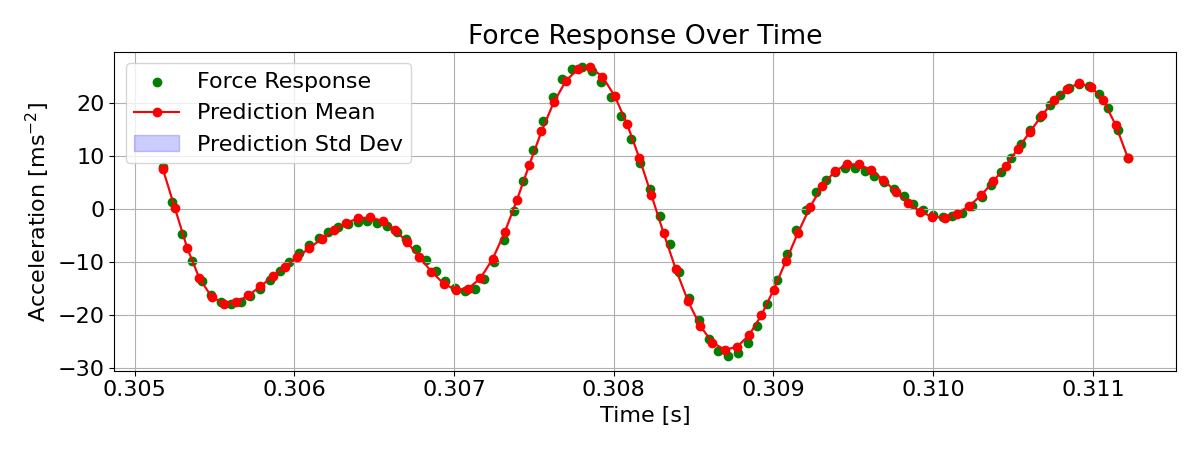
\includegraphics[width=1.0\linewidth]{figures/input-response-plot/input-response-plot.png}
%        \caption{The time series training data, and the mean and standard deviation of the GPs prediction of its latent function. Note that the prediction functions are continuous but must be evaluated at a discrete set of points in order to be plotted.}
%        \label{fig:input-response-plot}
%    \end{figure}

    \begin{figure}[h]
        \centering
        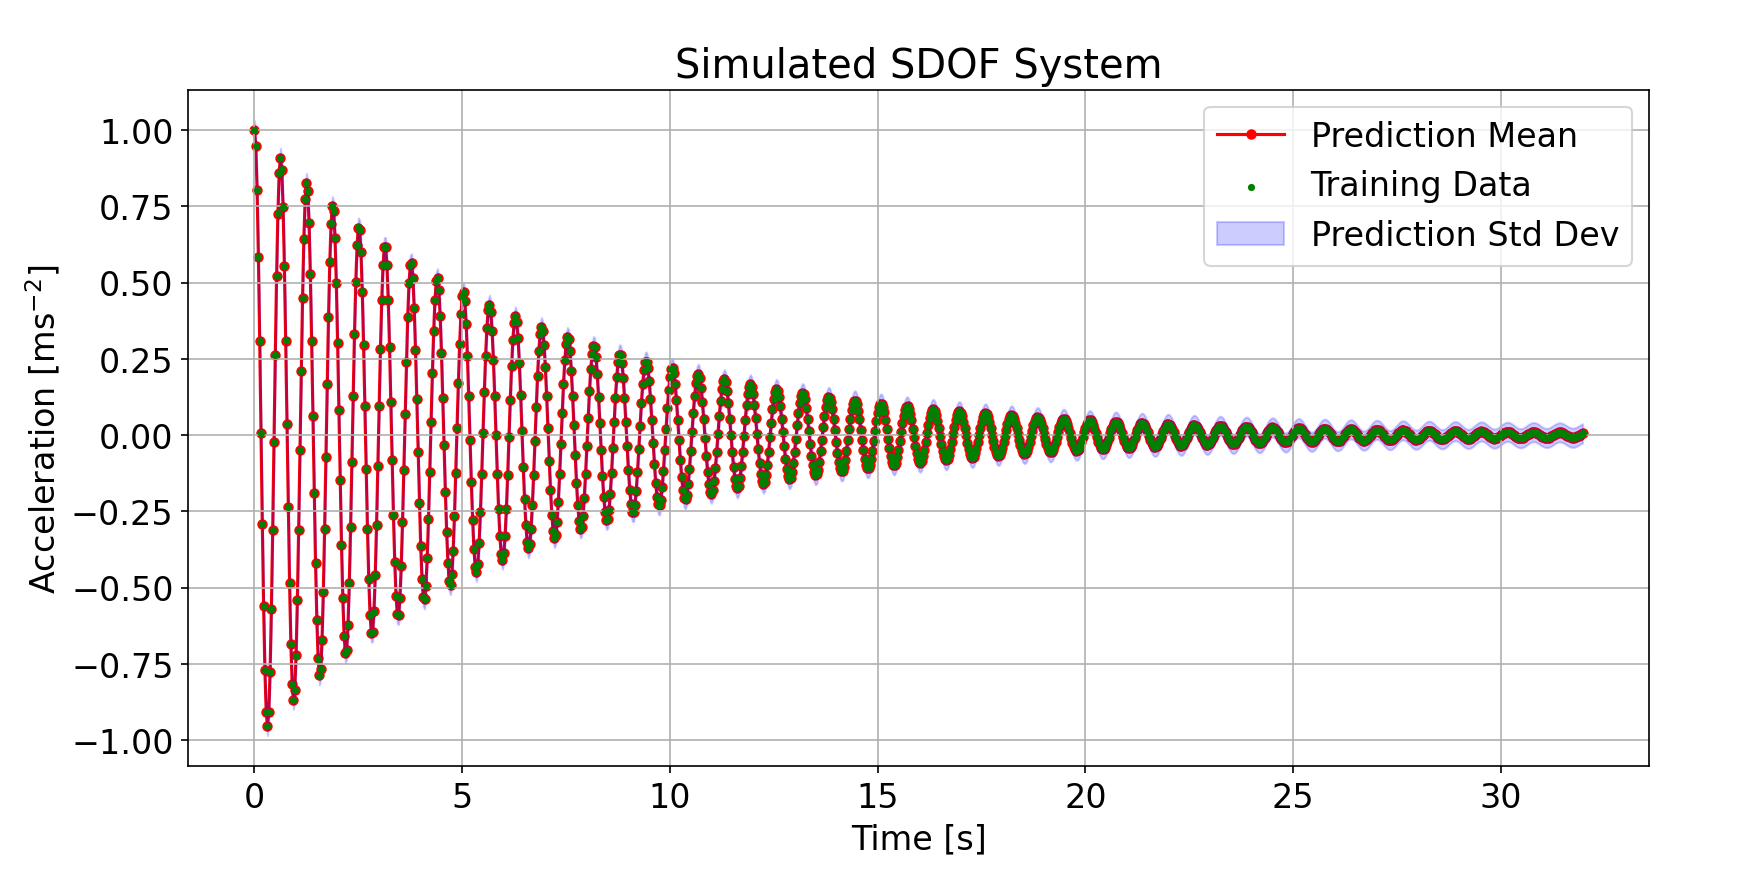
\includegraphics[width=1.0\linewidth]{figures/basic-data-time-domain/basic-data-time-domain.png}
        \caption{The basic training dataset of time domain acceleration of a simulated SDOF system consisting of $128$ datapoints at a sample rate of $32 \, Hz$ using system parameters $m = 1 \, kg$; $c = 0.3 \, Nsm^{-1}$; $k = 100 \, Nm^{-1}$ with no noise added, and the time domain prediction functions of the GP model fit to this data.}
        \label{fig:basic-data-time-domain}
    \end{figure}


    \subsection{The Kernel}
    A Squared Exponential Kernel~\cite{duvenaud2014kernel} was chosen to reflect the nature of the sample data, both of which are continuous and smooth, with no sudden jumps.
    In addition, the kernel has only two hyperparameters.
    This low number speeds up the hyperparameter optimisation process compared to alternative kernels.
    This function is defined in Equation~\ref{eq:se-kernel}

    \begin{equation}
        k(a,b) = \sigma^2 \exp\left(-\frac{(a - b)^2}{2l^2}\right) \label{eq:se-kernel}
    \end{equation}
    \nomenclature[L19]{$k(a,b)$}{The kernel function, evaluating the similarity of $a$ and $b$}
    \nomenclature[L02]{$a, b$}{Elements of vectors $\mathbf{A}, \mathbf{B}$ respectively}
    \nomenclature[L01]{$\mathbf{A}, \mathbf{B}$}{Vectors with elements $a, b$ - subscript indicates index of element}
    \nomenclature[G13]{$\sigma^2$}{The variance hyperparameter of the Squared Exponential Kernel}
    \nomenclature[L20]{$l$}{The length scale hyperparameter of the Squared Exponential Kernel}

    \noindent where $k(a,b)$ is the kernel function evaluated at elements $a_i$, $b_j$ of vectors $\mathbf{A}$, $\mathbf{B}$ respectively; $\sigma^2$ is the variance hyperparameter and $l$ is the length scale parameter.

%    The variance hyperparameter, $\sigma^2$, determines the average distance of the function away from its mean.
%    It is a simple scale factor present in all kernels.
%    Finally, length hyperparameter, $l$, determines how smooth or wiggly the function is, i.e., how fast the function can change direction.

    \subsection{Hyperparameter Optimisation}
    An algorithm was designed to optimise the hyperparameters of the kernel by minimising the Negative Log Marginal Likelihood (NLML), for which a method was written (see Appendix.~\ref{app:GPT}).
    It did this by modifying each hyperparameter randomly in turn and seeing if the NLML improved.
    This was repeated for up to $100$ iterations.

    Imagine if the hyperparameter was only updated if the new NLML was lower than the previous.
    Since the shape of a cost function can be complex and highly dimensional, the algorithm could have got stuck in local minima and have never found the global minimum.
    This would be analogous to a ball that ``tried'' to find the bottom of a valley by rolling directly downhill;
    if it got stuck in a small ditch half-way down the larger hill, it would never find the lowest point.

    Therefore, a mechanism was added to the algorithm to avoid this:
    If the new NLML was higher (i.e., worse) than the previous, the hyperparameter was maybe still updated, with a larger probability the closer the NLML was to the previous NLML\@.
    When the last iteration was complete, the lowest NLML of all the combinations hyperparameters was selected.
    This allowed the algorithm to explore after reaching a minimum to potentially find another part of the NLML function that was lower.

    \subsection{The Prediction Function}
    The prediction function was constructed, which accurately calculated the mean and standard deviation of the latent function as shown by the ``Prediction Mean'' and ``Prediction Std Dev'' plots in Figure~\ref{fig:basic-data-time-domain} respectively.
    The mean of each prediction point is calculated using Equation~\ref{eq:18.52} directly, whereas the standard deviation of each point uses only square root of the main diagonal of the covariance matrix resulting from Equation~\ref{eq:18.53}.
    In combination, this prediction function defines the probability distribution of the value of the latent function at any point, given the training data.
    Hence, when zero mean Gaussian noise with a standard deviation of $25 \, ms^{-2}$ was added to the training data, the standard deviation of the prediction became larger to take account for the uncertainty created by this noise, as shown in Figure~\ref{fig:noisy-data-time-domain}.

%    \begin{figure}[ht]
%%        \centering
%%        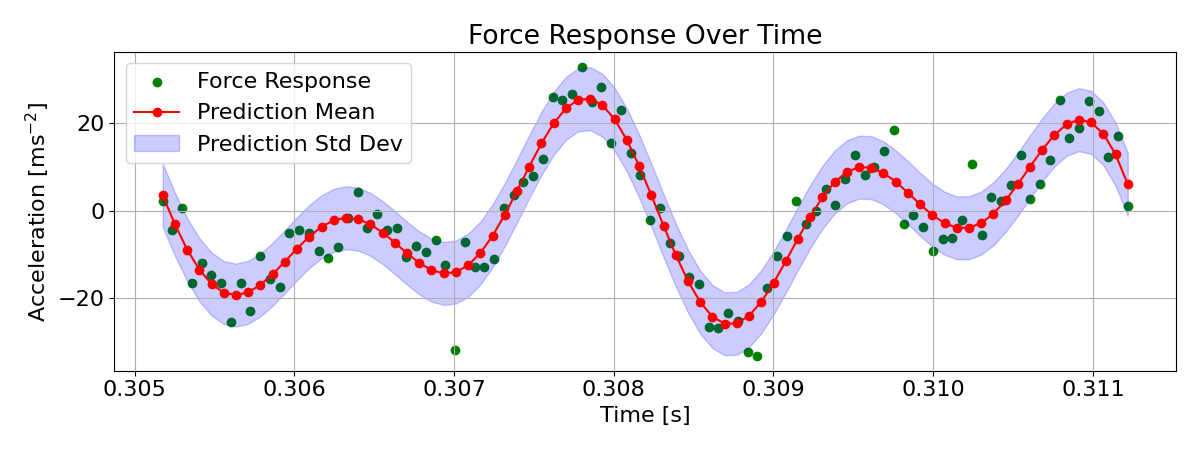
\includegraphics[width=1.0\linewidth]{figures/input-response-noise/input-response-noise.png}
%%        \caption{The mean and standard deviation of the prediction function of the GP when noise was added to the training data, showing that the standard deviation of the prediction increases when noise is added.}
%%        \label{fig:input-response-noise}
%%    \end{figure}


    \begin{figure}[h]
        \centering
        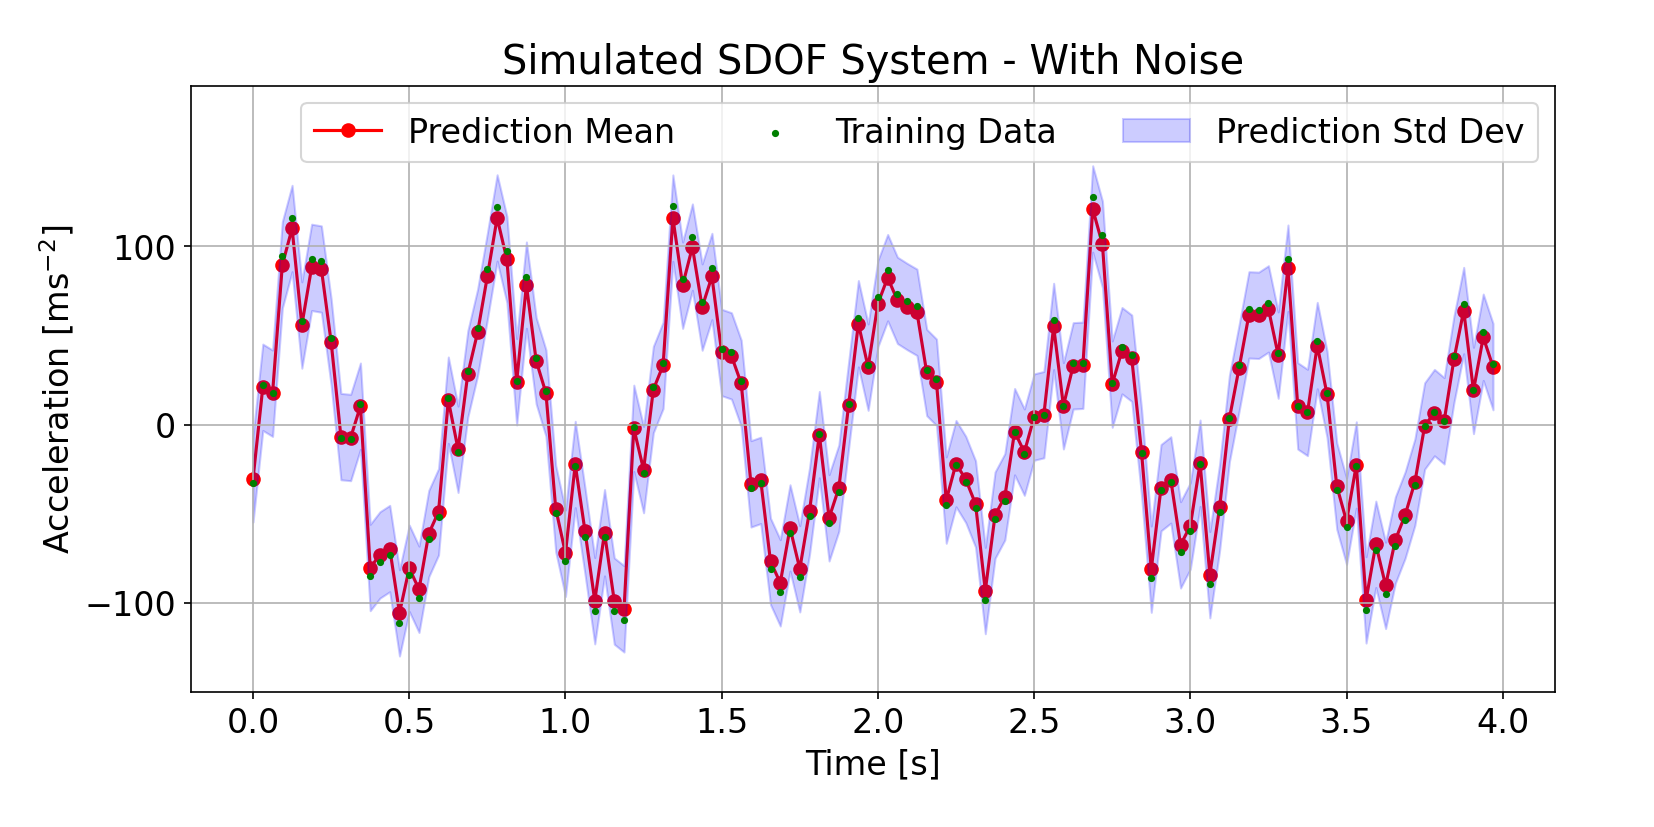
\includegraphics[width=1.0\linewidth]{figures/noisy-data-time-domain/noisy-data-time-domain.png}
        \caption{The mean and standard deviation of the prediction function of the GP when noise was added to the training data, showing that the standard deviation of the prediction increases.}
        \label{fig:noisy-data-time-domain}
    \end{figure}


    \section{Adjusting the Model for the Frequency Domain}

    \subsection{Finding the Posterior Mean of the Fourier Transform}
    Next, the function for the posterior mean of the Fourier transform was constructed, which could be evaluated at any set of points in the domain $(-\infty, \infty)$.
    This was done using a neat method described by Ambrogioni et al~\cite{Ambrogioni2018} which is equivalent to conditioning the joint distribution in Equation~\ref{eq:linear-trans}, but instead takes the Fourier transform of the time domain predictive mean function directly.
    Remarkably, this involved taking the Fourier transform of only the kernel, provided that the Fourier shift theorem was first applied to ensure that the kernel was a function of a single variable, as shown in Equation~\ref{eq:se-kernel-ft}

    \begin{equation}
        \mathcal{K}(\xi,0) = \frac{\sigma^2 l}{\sqrt{2 \pi}} \exp\left(-\frac{l^2 \xi^2}{2}\right) \label{eq:se-kernel-ft}
    \end{equation}

    \noindent where $\xi$ is the frequency and $\mathcal{K}(\xi,0)$ is the Fourier transform of the Squared Exponential Kernel function evaluated at $\xi$.

    For the mean function written in the form shown in Equation~\ref{eq:mean-sum-time-domain}

    \begin{equation}
        \mathbf{\mu}(t) = \sum_{k} w_k \, k(t,t_k) \label{eq:mean-sum-time-domain}
    \end{equation}

    \noindent where and $w_k$ is defined in Equation~\ref{eq:w_k}

    \begin{equation}
        w_k = \sum_{j} a_{kj} \, y_j \label{eq:w_k}
    \end{equation}
    \nomenclature[G065]{$\mu(t)$}{The mean function}

    \noindent where $a_{kj}$ is an element in matrix $\mathbf{A}$ defined in Equation~\ref{eq:A},

    \begin{equation}
         \mathbf{A} = (\mathbf{K}_{X,X} + \sigma^2_y \, \mathbf{I})^{-1} \label{eq:A}
    \end{equation}

    \noindent its Fourier transform is shown to be Equation~\ref{eq:mean-sum-freq-domain}.

    \begin{equation}
        \mathcal{F}[{\mu}](\xi) = \mathcal{K}(\xi,0) \sum_k w_k \, e^{- i \xi t_k} \label{eq:mean-sum-freq-domain}
    \end{equation}

    \subsection{Finding the Posterior Covariance of the Fourier Transform}

    The same steps can be used to derive the equation for the Fourier transform of the function for the main diagonal of the Covariance Matrix when written in the form shown in Equation~\ref{eq:var-sum-time-domain}

    \begin{equation}
        \Sigma(t) = k(t,t) - \sum_k v_k \, k(t,t_k) \label{eq:var-sum-time-domain}
    \end{equation}
    \nomenclature[G145]{$\Sigma(t, t)$}{The covariance function of the Gaussian Process in the time domain}
    \noindent where $v_k$ is defined in Equation~\ref{eq:v_k}

    \begin{equation}
        v_k = \sum_j a_{kj} \, k(t,t_j) \label{eq:v_k}
    \end{equation}

    \noindent where $t_j$ is the $j^{th}$ element in $\mathbf{X}$.

    The resulting Fourier transform can be written as shown in Equation~\ref{eq:var-sum-freq-domain}

%    \begin{equation}
%        \mathcal{F}[\Sigma](\xi, \xi) = \frac{1}{2 \pi} e^{- i \xi^2} k(- \xi,0)  - \sum_k \sum_j a_{kj} \, e^{-i \xi (t_j - t_k)} \mathcal{K}(\xi,0)^2 \label{eq:var-sum-freq-domain}
%    \end{equation}

    \begin{equation}
        \mathcal{F}[\Sigma](\xi, \xi) = \mathcal{K}(\xi,0) \delta(\xi - \xi)  - \sum_k \sum_j a_{kj} \, e^{-i \xi (t_j + t_k)} \mathcal{K}(\xi,0)^2 \label{eq:var-sum-freq-domain}
    \end{equation}
    \nomenclature[G01]{$\delta$}{The Dirac delta function}

    \noindent where $\delta$ is the Dirac delta function, which ensures that the two inputs are equal.

    Only the main diagonal was computed because this is all that is required to plot the standard deviation of the output predictions (which is the square root of the covariance), and because hyperparameter training (which would require the full matrix) was completed in the time domain already.
    This decreased the compute requirements significantly, from $O(N^2)$ to $O(N)$, where N is the number of frequency predictions required.

    \section{Results and Discussion}
    After this Gaussian Process Model was complete, it could then be set up and used in a variety of test cases to explore its advantages and disadvantages versus the Fast Fourier Transform.
    The dataset used the same model as in Figure~\ref{fig:basic-data-time-domain}, but the number of datapoints was extended to 1024 (at the same sample rate of $32 \, Hz$) to provide more information, allowing for more accurate results.

    \subsection{The Basic Dataset}
    \subsubsection{Accuracy of the Fourier Transform} \label{Acc}
    Initially, no noise was added in order to verify the new approach of computing the Fourier transform.
    Since the dataset was simulated using known parameters, the exact Fourier transform of the latent function could be calculated analytically.
    This could be used to test the accuracy of the GP model, using the performance of the FFT (with a Hanning window) on the same system as a benchmark.
    Here, the posterior mean of the GP's Fourier transform, as well as the FFT and the analytical Fourier transform were calculated.
    Since the Fourier transform is complex, to show it fully in graph form it must be broken down into two components - either into its magnitude and phase, or into its real and imaginary parts.
    Both representations are shown in Figure~\ref{fig:basic-data-freq-domain} for each of the three variants of the Fourier transform.

    \afterpage{
        \clearpage
        \begin{landscape}
            \begin{figure}[p]
                \centering
                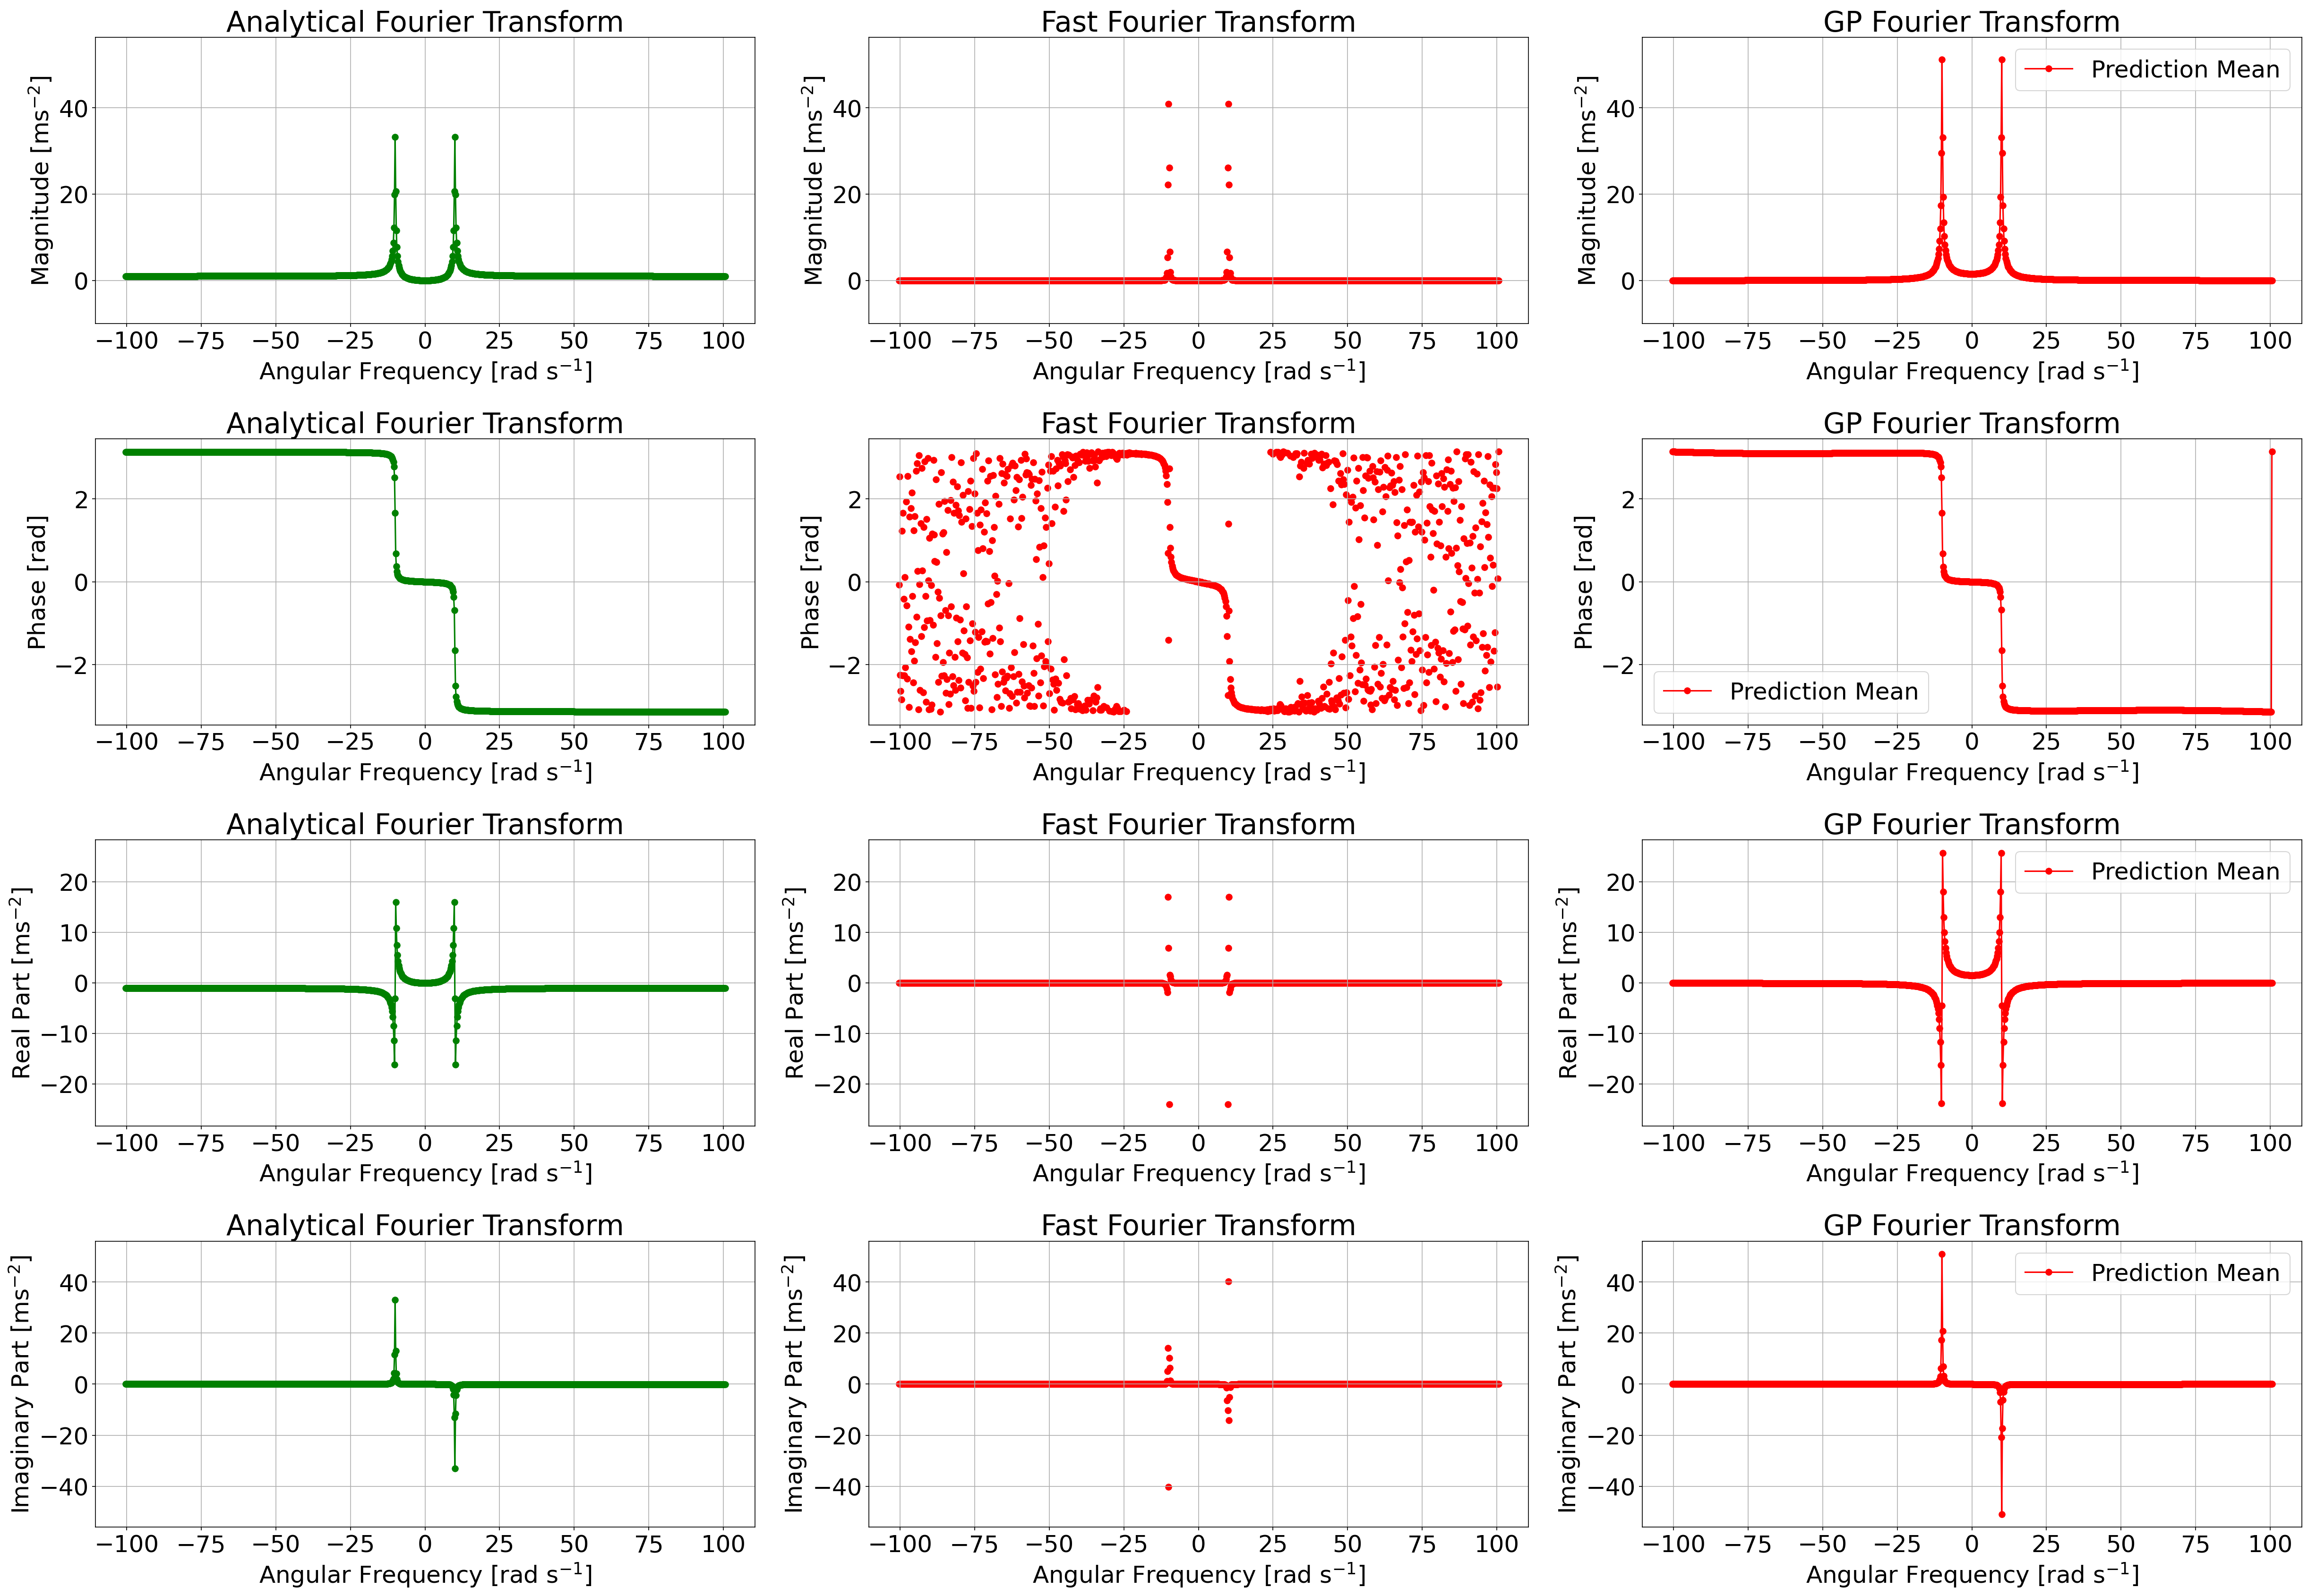
\includegraphics[width=\linewidth]{figures/basic-data-freq-domain/basic-data-freq-domain.png}
                \caption{The analytical Fourier transform, FFT and the posterior mean of the GP's Fourier transform for the basic dataset of the SDOF system without noise, broken down into the magnitude and phase components, as well as the real and imaginary components.}
                \label{fig:basic-data-freq-domain}
            \end{figure}
        \end{landscape}
        \clearpage
    }

    To verify the model, the properties of the peak were compared to the exact simulated value for each.
    From observation of the magnitude plots, the GP Fourier transform seems to more smoothly reach the peak, which resembles the shape of the analytical Fourier transform more closely than the FFT.
    This suggests that it captures information relating to damping better, likely because the FFT's Hanning window would distort the signal's exponential decay in the time domain from the damping dissipating energy over time.
    Since the mean of the GP was sampled in the frequency domain in the same places as the FFT, the angular frequency of the peak - as measured by the sample with the largest magnitude - was identical, $10.01 \, rad \, s^{-1}$, within one sample interval of the analytical peak of $10.00 \, rad \, s^{-1}$.
    The percentage errors in the magnitude of the peaks were $22.7 \, \%$ and $53.5 \, \%$ for the FFT and GP model respectively.

    Next, the Mean Squared Error (MSE) was used to compare the accuracy (lower is better) of each of the FFT and the posterior mean of the GP's Fourier transform with respect to the analytically exact Fourier transform.
    This algorithm finds the average of the squares of the differences between the points at each index position of two series, as shown in Equation~\ref{eq:mse}.

    \begin{equation}
        \text{MSE} = \frac{1}{n} \sum_{i=1}^{n} (a_i - b_i)^2 \label{eq:mse}
    \end{equation}

    \noindent where $a_i$, $b_i$ are the values of vectors $\mathbf{A}$, $\mathbf{B}$ at index i.

    The MSE for the magnitude component, as well as the real and imaginary parts of each of the two numerical methods is shown in Table~\ref{tab:basic-mse}, where the error of the magnitude GP model's Fourier transform was $1.22$ times larger than that of the FFT, but error real and imaginary parts were $4.42$ and $12.66$ times smaller respectively.

    \begin{table}[H]
        \centering % This centers the table on the page
        \setlength{\arrayrulewidth}{1pt} % Sets the thickness of the table borders
        \begin{tabular}{|c|c|c|} % 'c' for centered columns, '|' for vertical lines between columns
            \hline
            Basic Dataset & FFT & GP FT Mean \\ % Titles for the columns
            \hline
            Magnitude MSE [ms$^{-2}$] & $2.09$ & $2.55$ \\
            \hline
            Real Part MSE [ms$^{-2}$] & $7.59$ & $1.72$ \\
            \hline
            Imag Part MSE [ms$^{-2}$] & $10.57$ & $0.83$ \\
            \hline
        \end{tabular}
        \caption{A table showing the Mean Squared Error (MSE) for the components of both the FFT, and the posterior mean of the GP's Fourier transform when compared to the analytically exact Fourier transform for the basic dataset.}
        \label{tab:basic-mse}
    \end{table}

    Note that the MSE of the phase was not computed because numerical instabilities had a large effect in its values when the real and imaginary components were near zero, so it wouldn't have been meaningful.
    But overall, the performance of the GP model was comparable to the FFT, since neither was superior in every metric.
    Therefore, the GP model was shown to be a valid alternative to the FFT\@.

    \subsection{Robustness to Noise}
    The robustness to noise was tested (Objective~\ref{noise-resilience}) by calculating the MSE of the two methods when zero mean Gaussian noise with a standard deviation of $25 \, ms^{-2}$ was added to the signal.
    The components of the Fourier transforms are shown in Figure~\ref{fig:noisy-data-freq-domain}.

    \afterpage{
        \begin{landscape}
            \begin{figure}[p]
                \centering
                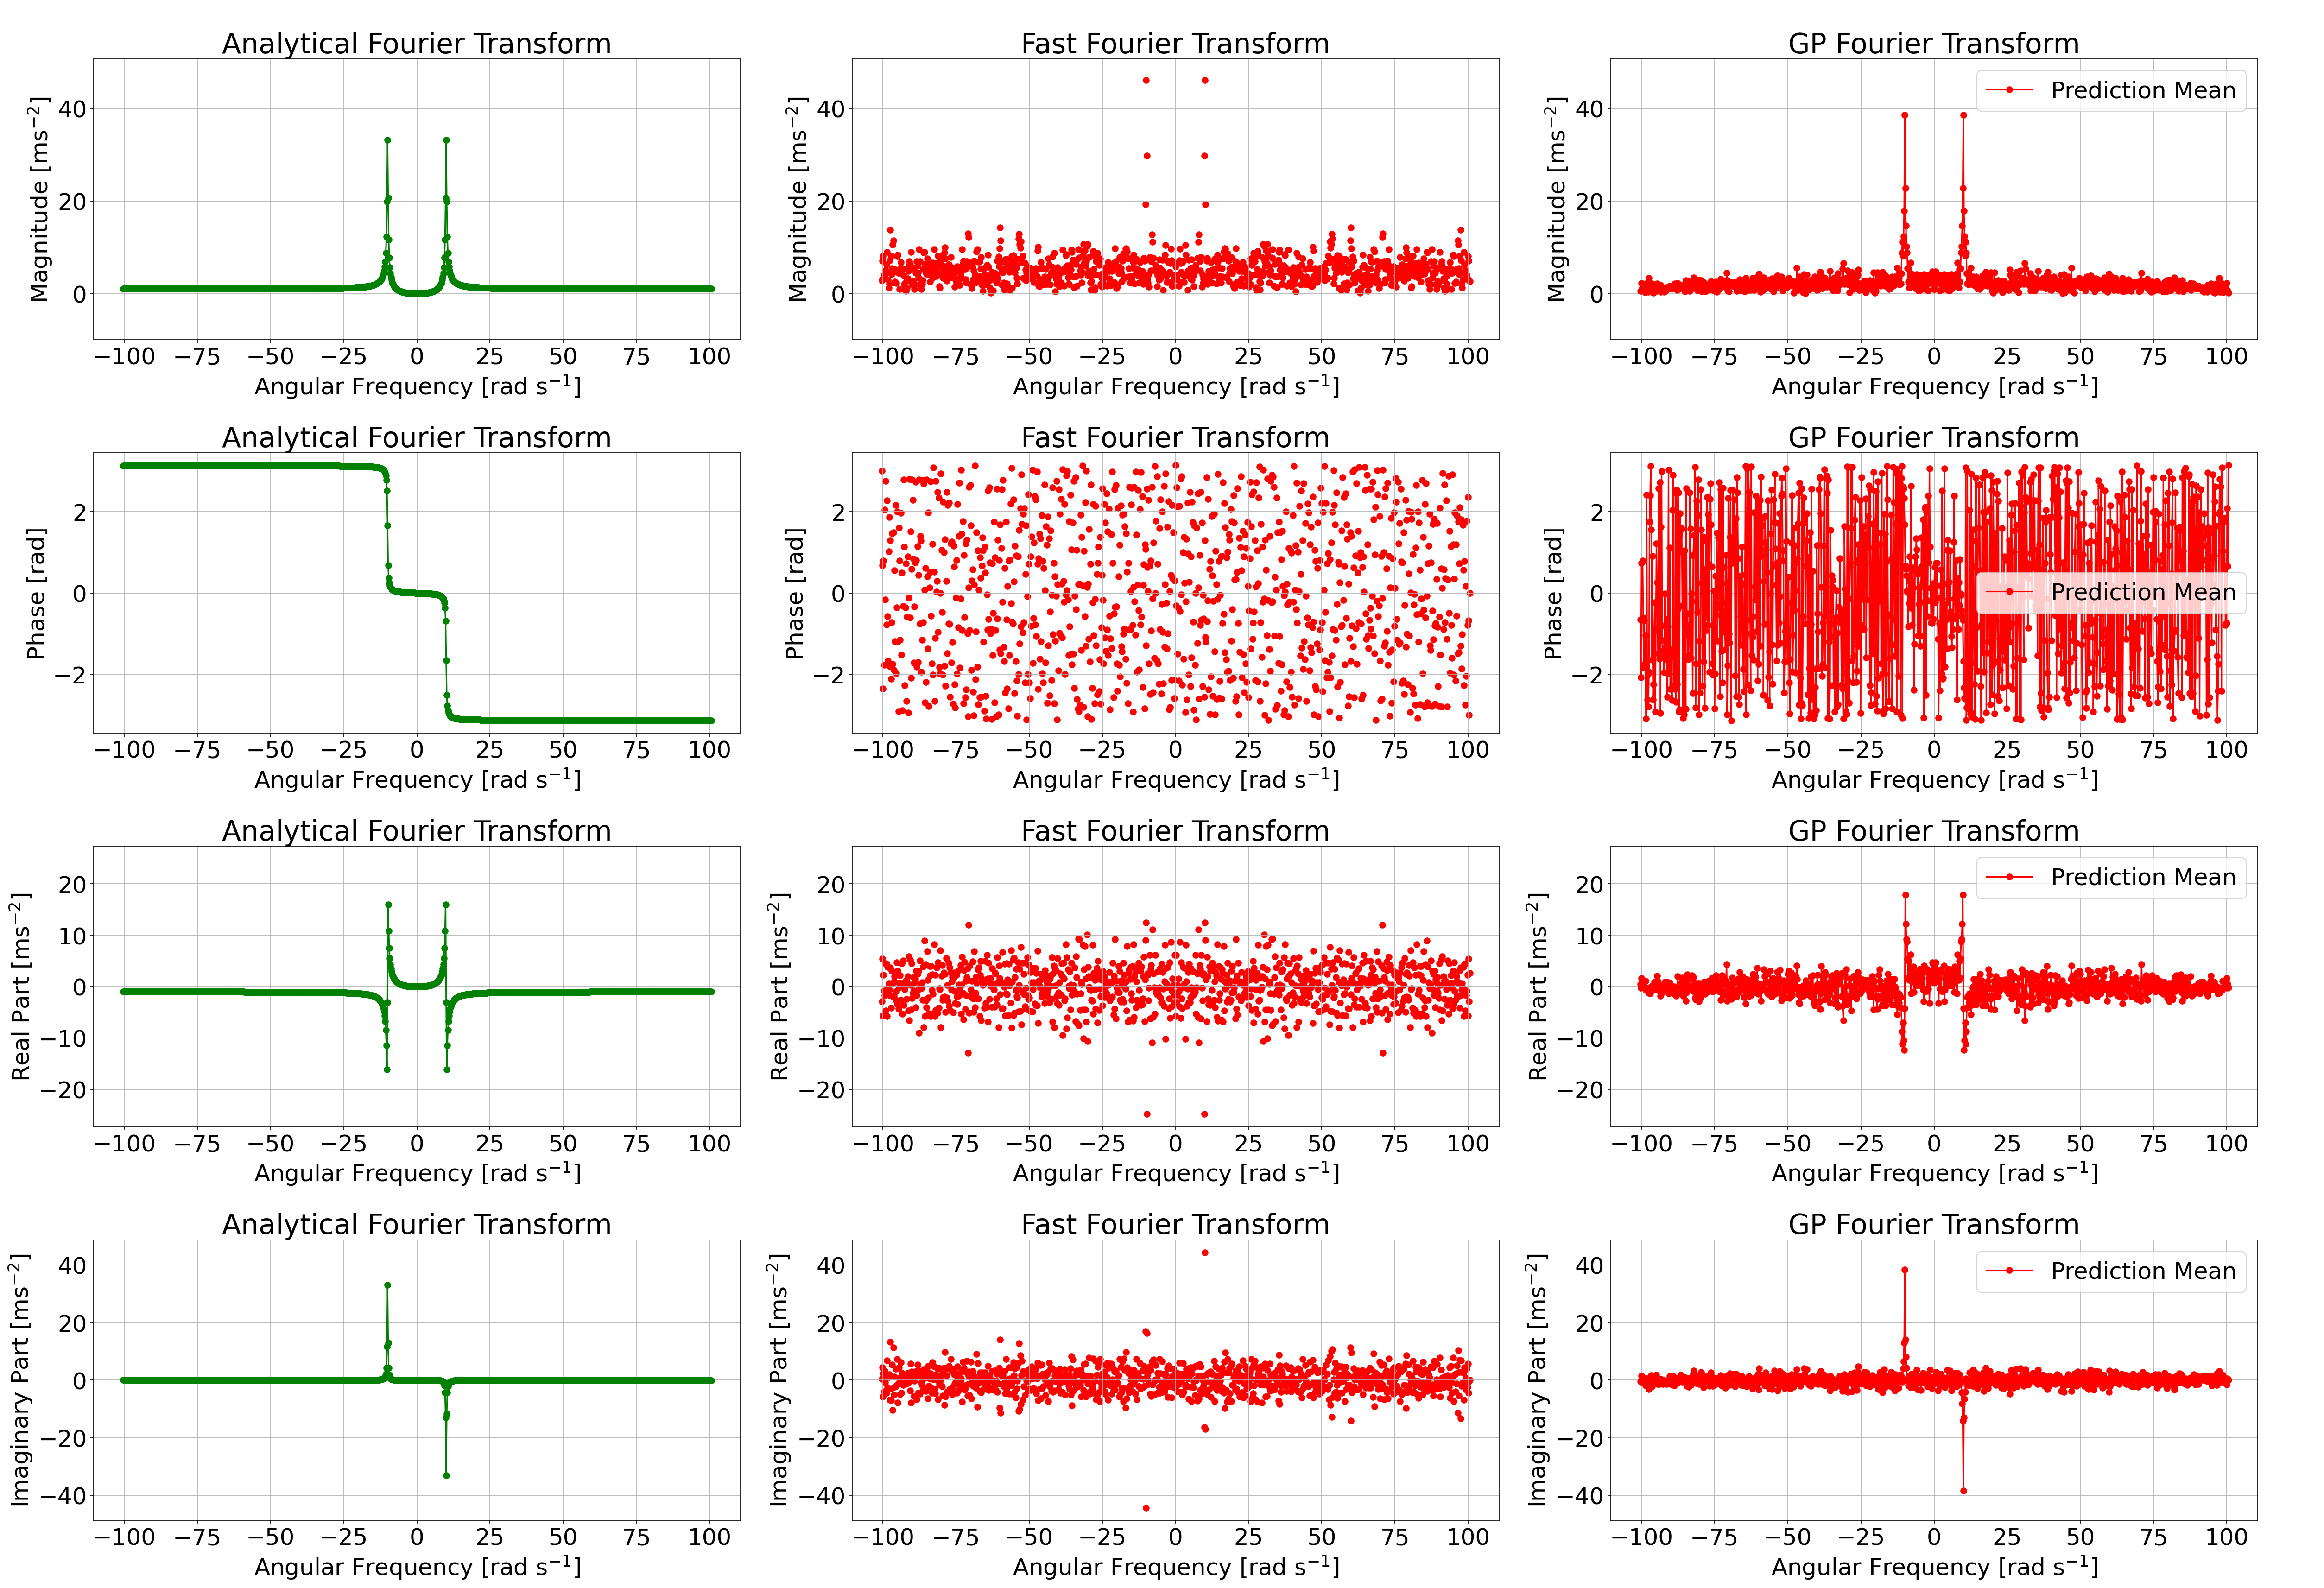
\includegraphics[width=\linewidth]{figures/noisy-data-freq-domain/noisy-data-freq-domain.png}
                \caption{The analytical Fourier transform, FFT and the the posterior mean of the GP's Fourier transform when Gaussian noise with a standard deviation of $25 \, ms^{-2}$ was added to the signal, broken down into the magnitude and phase components, as well as the real and imaginary components.}
                \label{fig:noisy-data-freq-domain}
            \end{figure}
        \end{landscape}
    }

    Table~\ref{tab:response-noise} shows that the GP model performed significantly better here, with the error of the magnitude, and real and imaginary parts of the GP model's Fourier transform being $9.66$, $6.48$ and $11.64$ times smaller than the FFT respectively.

    \begin{table}[ht!]
        \centering % This centers the table on the page
        \setlength{\arrayrulewidth}{1pt} % Sets the thickness of the table borders
        \begin{tabular}{|c|c|c|} % 'c' for centered columns, '|' for vertical lines between columns
            \hline
            Noisy Dataset & FFT & GP FT Mean \\ % Titles for the columns
            \hline
            Magnitude MSE [ms$^{-2}$] & $22.80$ & $2.36$ \\
            \hline
            Real Part MSE [ms$^{-2}$] & $22.88$ & $3.53$ \\
            \hline
            Imag Part MSE [ms$^{-2}$] & $27.94$ & $2.40$ \\
            \hline
        \end{tabular}
        \caption{A table showing the Mean Squared Error (MSE) for the components of both the FFT, and the posterior mean of the GP's Fourier transform when compared to the analytically exact Fourier transform when Gaussian noise with a standard deviation of $25 \, ms^{-2}$ was added to the signal.}
        \label{tab:response-noise}
    \end{table}

    Furthermore, the magnitude of the peak was found more accurately by the GP model in this case, with a percentage error of $15.8 \, \%$ versus $38.1 \, \%$ for the FFT, with no change in the angular frequency of the peak for either method.

    Since real world data always contains noise, this Fourier transform that is more robust to noise would have widespread benefits in mechanical engineering because it would allow for more accurate Frequency Response Functions (FRFs) of structures, and therefore more accurate identification of system properties.
    After the FRF of a structure such as a wind turbine tower is determined, it can be evaluated with the same forces that the system is expected to experience to predict the maximum amplitude of vibration expected during its lifetime.
    If this is excessive, the system is at risk of mechanical failure or high cycle fatigue, so the design must be changed to prevent this.
    For example, the mass could be changed to move the resonant frequency (indicated by the angular frequency of a peak) away from the expected forcing frequency, reducing the expected amplitude of oscillation.
    Alternately, damping could be added to smooth out the resonance peak, reducing its amplitude.
    Therefore, being able to more accurately determine the FRF and the properties of its peaks through this new GP method would be beneficial in the design process because one would be able to more accurately determine how the design needs to change to reduce the risk of failure to acceptable levels.

    \subsection{Non-Uniform Sampling of Frequency Domain}
    Since the Fourier transform is a continuous function, it can be sampled at any set of points in the domain $(-\infty, \infty)$.
     So, taking the basic dataset and clustering an additional $100$ samples of the spectrum of the GP in the interval of $1 \, rad \, s^{-1}$ containing the peak was able to improve the error in the calculation of the angular frequency of the peak from the same as the FFT ($0.0149 \, rad \, s^{-1}$) down to $0.0039 \, rad \, s^{-1} $.
    However, the error in the magnitude of the peak ($54.2 \, \%$) was still larger than that of the FFT ($22.68 \, \%$).

    If the time domain GP was an exact fit to the latent function, as the interval of angular frequency between samples around the peak tended to zero, so would this error.
    This is not possible with the FFT because the location of the spectrum samples are determined by the time domain samples, both of which must be evenly spaced, meaning that spectrum samples could fall either side of a sharp peak, which creates an uncertainty of $\pm$ half the sample interval.

    Furthermore, since the frequency interval is inversely proportional to the total time period, the difference between the error of the peak of the GP model and the FFT is more pronounced for data over a shorter time period.
    For instance, using only the first $64$ points of the same dataset gave the FFT an error in the angular frequency of the peak of $0.574 \, rad \, s^{-1}$ versus $0.054 \, rad \, s^{-1}$ for the GP model - a significant improvement.
    In addition, the error in the magnitude of the peak ($60.64 \, \%$) even beat that of the FFT ($685 \, \%$), which performed very poorly for this short dataset.
    This means that this proposed GP model may be better suited for use cases in which there is limited time for testing, such as in the aforementioned example of hypersonic wind tunnel tests of scramjets.

    \subsection{Non-Uniform Sampling of the Time Domain and Overcoming Aliasing and the Nyquist Limit}
    Similarly, the time domain input data need not be uniformly spaced in order to fit the GP\@.
    This would allow the model to be used to find the Fourier transform of datasets with missing data, which may occur, for example, if an accelerometer placed on a gas turbine engine during a test failed to transmit data for a period of time due to a loose connection.
    If enough data was still present to faithfully represent the system, the GP would not be significantly affected which would allow the test data to still be used.
    On the other hand, if the standard FFT was used, the test would either need to repeated at added cost, or additional steps would need to be taken to preprocess the data, adding complication.

    However, more impressively, this feature allows frequencies to be detected that would be above the Nyquist limit for the FFT with the same number of datapoints over the same sampling period.
    This is because for a given time period and number of samples available, many can be bunched in a portion of the time period in order to capture the behaviour of high frequency signal components, leaving a few points over the full period of time to capture well damping information related to the exponential decay of the signal.
    For example, when increasing the model stiffness to $k = 20,000 \, Nm^{-1}$, and fitting the GP to datapoints sampled over the period at random points in a triangular distribution, it was able to detect the true peak at $141.4 \, rad \, s^{-1}$ with an error of less than $0.1 \, rad \, s^{-1}$.
    The FFT of an equivalent dataset containing the same number of datapoints sampled evenly over the same time period for the same system peaked at $59.7 \, rad \, s^{-1}$, which is an artifact of aliasing caused by the true peak being reflected about the Nyquist limit of $100.5 \, rad \, s^{-1}$.

    This feature of the GP model could be used in contexts where the identification of high frequencies as well as damping information is required, yet there are tight constraints on memory such as in the aerospace industry.
    Here, a microsatellite must monitor the heavy vibration it experiences on ascent to orbit to ensure the components onboard haven't exceeded their structural limits, which could indicate damage.
    This would likely include Fourier analysis of accelerometer data to monitor vibration in the frequency domain.
    However, the memory available to do this is limited because storage capacity has weight, every gram of which significantly increases the fuel requirements and cost to get the satellite to orbit.
    Therefore, this ability to detect higher frequencies than an equivalent FFT using the same amount of data and memory would be valuable here.

    \subsection{The Posterior Covariance of the Fourier Transform}
    The spectrum prediction of the GP model at a given angular frequency is a Gaussian distribution, with a standard deviation around the mean derived from the posterior covariance of the GP's Fourier Transform as shown in Figure~\ref{fig:stdv-plot}.
    Here, the standard deviation is largest around $0 \, rad \, s^{-1}$, and tapers off for higher frequencies.
    This makes intuitive sense because there are fewer cycles of the lower frequency components in a given time period, so there is less information available to use to detect them.

    \begin{figure}[!htb]
        \centering
        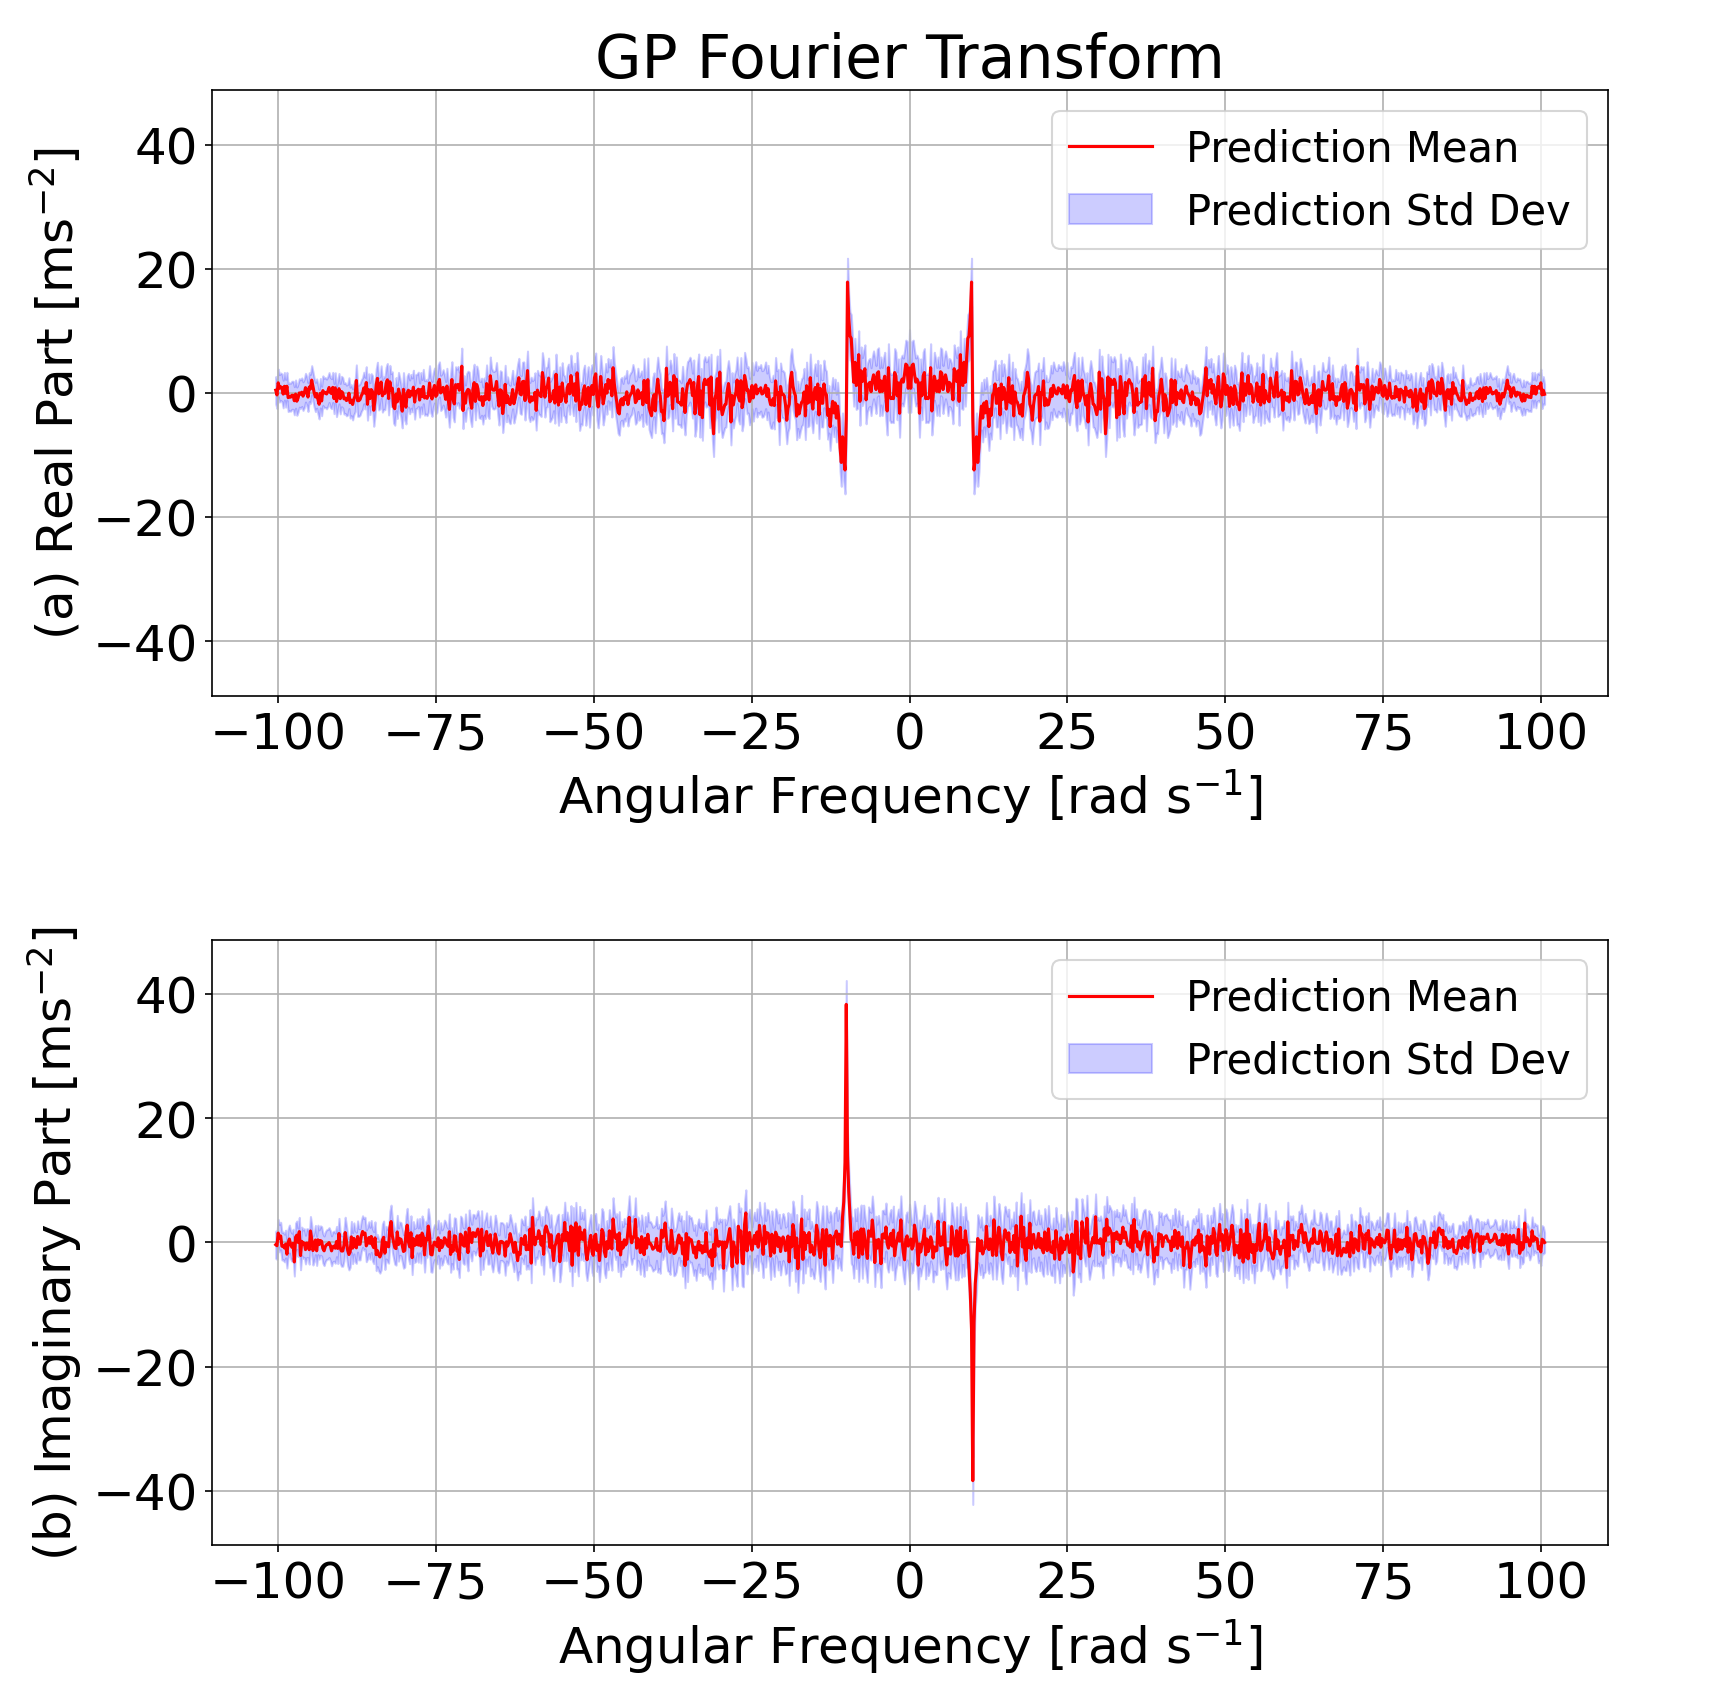
\includegraphics[width=\linewidth]{figures/stdv-plot/stdv-plot.png}
        \caption{The real (a) and imaginary (b) components of the frequency domain prediction function of the GP including the standard deviation for the noisy dataset.}
        \label{fig:stdv-plot}
    \end{figure}

    In the automotive industry, a piston connecting (``con'') rod in an internal combustion engine undergoes heavy vibration of very many cycles (twice for each revolution of a four-stroke engine), so fatigue analysis is crucial to ensure that it does not fail from crack formation and propagation before the end of the design life of the vehicle.
    Since they are typically made of a ferrous alloy such as forged steel, they have a fatigue limit~\cite{RoymechFatigue}, which is a distinct stress level for a given frequency below which failure from fatigue will not occur - even from an infinite number of loading cycles~\cite{BeerJohnston1992}.
    This stress level can be calculated from experimental acceleration data, and therefore it can be shown that the stress on the con rod is below the fatigue limit by showing that the magnitude of acceleration across the range of frequencies is below its corresponding limit.
    Testing this would be valuable because one could show that the con rod will not fail from fatigue if the test passes.

    However, if the FFT was used, even if the nominal value calculated was below its limit, the uncertainty interval would be unknown and so it would still be unclear whether the upper bound of the range of possible values is above the fatigue limit.
    Therefore, one could not confidently conclude that the system is below the fatigue limit without a conservative factor of safety.

    In contrast, ``rather than relying on large factors of safety to account for uncertainty''~\cite{Rogers2023} which could add unnecessary weight to overly strengthen the component, the uncertainty information is encoded in the posterior covariance of the GP's Fourier transform.
    Therefore, it would be possible to calculate a confidence interval of, say, $3 \sigma$ for the prediction, and if this is entirely below the fatigue limit, one can conclude that the component passes the test without the need for a conservative safety factor, increasing the performance of the engine.

    \section{Directions for Future Work}
    \subsection{Alternative Kernels}
    Looking at Figure~\ref{fig:noisy-data-time-domain}, the posterior mean appears to overfit the training data since it jumps from training point to training point, including the noise instead of only fitting to the underlying latent function that varies smoothly.
    If a different kernel was used that was better suited to the expected shape of the data, the posterior mean may fit the latent function better.
    For instance, a periodic kernel would be well suited since the latent function is cyclic in nature.
    To also capture the exponential decay over time, a ``compound'' kernel could be formed by multiplying it with the Squared Exponential Kernel~\cite{duvenaud2014kernel}.
    Although the posterior mean of the GP's Fourier transform showed good robustness to noise versus the FFT, if this compound kernel eliminated overfitting, this could significantly improve the robustness to noise of the posterior mean of the Fourier transform further.
    However, if the kernel is too complicated, the required analytical Fourier transform of the kernel may become intractable.

    \subsection{Computation Time and Scaling to Large Data}
    Although this new Gaussian Process (GP) method of performing the Fourier transform is promising, one major disadvantage of this GP model is it struggles to scale large datasets due to the long computation time, especially the hyperparameter training phase since it is of $O(N^3)$\nomenclature[L24]{$O()$}{Big O notation, used to describe the complexity - or ``Order'' of an algorithm}, which is poor compared to $O(N \log{N})$ for the Fast Fourier Transform (FFT)~\cite{murphy2023probabilistic}.
    This means that the model handles poorly datasets consisting of more than a few thousand points, and even at this scale, fitting the GP to the time domain then converting this to the frequency domain takes several orders of magnitude longer ($0.84 \, s$) than the time the FFT ($7.5 \times 10^{-5} \, s$) takes to run.
    This performance is poor considering that it is not uncommon to need to work with datasets consisting of up to a million datapoints in industry, such as during a tap test for modal analysis of a turbine blade, for which the GP model in its current state would be impractical due to the excessive time and cost computational resources that would be required.

    To address this, a sparse GP approximation could be employed to allow both the NLML and prediction functions to scale to large data.
    One type of sparse GP approximation is the Fully Independent Training Conditional (FITC)~\cite{q-candela}.
    This would reduce the complexity of the training phase from $O(N^3)$ to $O(MN^2)$, where M is a set of inducing points chosen to be a subset of the original training points, and $N \gg M$. \nomenclature[L21]{$M$}{The number of inducing points in Sparse GP}
    After this is complete, the hyperparameters could be optimised and the GP could be fit for functions containing more than $10,000$ data points in a significantly reduced computation time.
    However, in practice an implementation could not be found that was numerically stable enough for the NLML values to match the basic GP when the set of inducing points is exactly the same as the test dataset, which they should.
    This led to poor convergence and was likely due to the matrix operations involved such as determinants and inverses that can be unstable for large matrices.

    To progress further, one may have better performance implementing an alternative sparse GP approximation such as the Variational Free Energy (VFE) approach, which works by approximating the posterior distribution, rather than the prior~\cite{murphy2023probabilistic}.

%    \subsection{and another subsection}
%    \textcolor{red}{ New kernel types; multi degree of freedom / dimension GP's!!!!; different solver types? etc.}

    \section{Conclusion}
    Overall, this paper explored a new paradigm of ``probabilistic numerics'' over traditional numerical methods that allowed the Fourier transform to be performed through the use of a Gaussian Process (GP) machine learning model.
    This model showed significantly better robustness to noise compared to the industry standard Fast Fourier Transform (FFT), exhibiting an improved Mean Squared Error in magnitude versus the true analytical Fourier transform by a factor of $9.66$.

    The identification of dynamic systems often uses the ``Frequency Response Function'', which relies on the ``Fourier transform'' to convert data from a function of time to a function of frequency.
    Therefore, the model could allow dynamic systems to be identified more accurately in across industry where data is noisy, from aviation to renewable power generation.
    This would help to design structures that last longer before failing from fatigue, and that are less likely to fail structurally from excessive excitation under external forces.

    Furthermore, the model had several promising features that made it more versatile in this context.
    Most notably, the fact that the time domain input data need not be evenly spaced enabled it to detect frequencies that would be above the Nyquist limit of an equivalent FFT of the same number of datapoints sampled evenly across the same time period.
    This makes the model most suitable in industrial contexts where there are constraints to the amount of data that can be collected due to cost, availability, or limited memory.

    However, the computational speed of this GP model is currently orders of magnitude slower than the FFT, so before it can be a viable alternative in practice, it would need development to allow it to scale better to large datasets.

    \FloatBarrier

    \newpage
    \printbibliography
    \addcontentsline{toc}{section}{References}
    \newpage
    \appendix
\section{The use of generative AI (ChatGPT)}
OpenAI's ChatGPT interface, powered by the GPT-4 large language model, was used to implement the Negative Log Marginal Likelihood (NLML) method in my code in a specific way to ensure numerical stability though the use of the ``Cholesky decomposition''.
The prompt and output is provided in Figure~\ref{fig:chat-NLML}.
\begin{figure}[htbp]
    \centering
    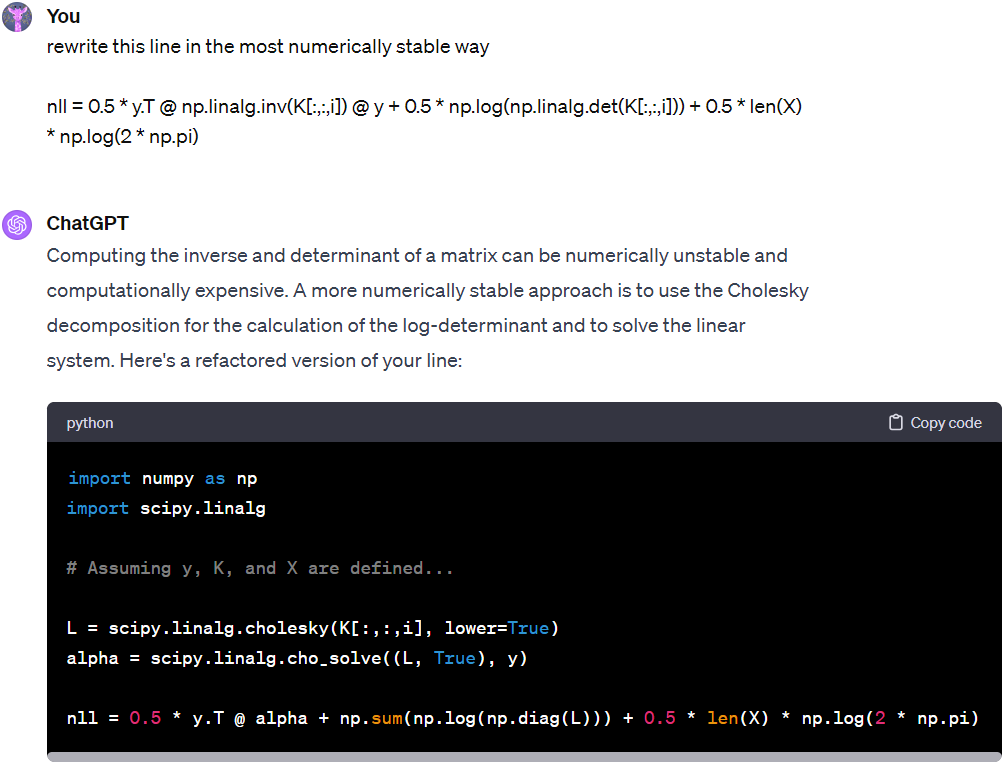
\includegraphics[width=1\linewidth]{figures/chat-NLML/chat-NLML.png}
    \caption{ChatGPT prompt and output providing a way to compute the NLML that is faster and more numerically stable}
    \label{fig:chat-NLML}
\end{figure}

\FloatBarrier

In order to ensure that this function was valid, its implementation was confirmed by the relevant literature~\cite{murphy2023probabilistic}~(Section 18.3.6).
After which, this function was simplified and adapted into that it could be to be added to the $gp\_model$ class as a method, and so that it would work with the way the input data was formatted, as shown in Listing~\ref{1st:NLML}

\begin{lstlisting}[caption={Method used to calculate the Negative Log Marginal Likelihood (NLML).} language=Python,label={lst:NLML}]
    def compute_nlml(self, hyperparameters):
    self.update_hyperparameters_and_debug(hyperparameters)
    self.reshape_X_and_y()

    if self.gp_algo == 'cholesky':
        K = self.gp_kernel.compute_kernel(self.X, self.X)
        K += np.repeat(np.array(np.eye(len(self.X)) * 1e-3)[:,:, np.newaxis], self.X.shape[1], axis=2)
        debug_K = np.squeeze(K)
        L = scipy.linalg.cholesky(K[:, :, 0], lower=True)
        n = len(self.y)
        one_vector = np.ones(n)
        y_adj = self.y - self.y_mean

        alpha = scipy.linalg.cho_solve((L, True), y_adj)

        term_1_c = (0.5 * y_adj.T @ alpha).item()
        term_2_c = np.sum(np.log(np.diag(L)))
        term_3_c = 0.5 * n * np.log(2 * np.pi)

        nlml = term_1_c + term_2_c + term_3_c

        out_c = {
            'nlml': nlml,
            'term_1': term_1_c,
            'term_2': term_2_c,
            'term_3': term_3_c
        }

        return out_c

\end{lstlisting}




\end{document}